\documentclass{article}
\usepackage{hyperref}
\usepackage{comment}
\usepackage{longtable}
\usepackage{array}
\usepackage{amssymb}
\usepackage{graphicx}
\usepackage{fancyhdr}
\usepackage[T1]{fontenc}
\usepackage[italian]{babel}
\usepackage{amsmath}
\usepackage{enumitem}
\usepackage{sourcecodepro}
\usepackage{tikz} %copertina
\usetikzlibrary{shapes.geometric, calc} %copertina
\usepackage{xcolor} %copertina
\usepackage{tcolorbox}

%\usepackage[scaled=0.8]{luximono}
%\usepackage{geometry}

\def\code#1{\texttt{#1}}



\usepackage{listings} %sql
\lstset{
    language=C++, 
    basicstyle=\small\ttfamily,
    numbers=left, 
    numberstyle=\tiny, 
    frame=line,
    keywordstyle=\color{blue},
    commentstyle=\color{purple},
    stringstyle=\color{orange},
    %identifierstyle=\color{black},
    %numberstyle=\tiny\color{black},
    breaklines=true,
    linewidth=1.185\linewidth
}




\begin{document}

\begin{tikzpicture}[overlay,remember picture]

\definecolor{Dandelion}{RGB}{240, 225, 48} % Esempio di definizione del colore Dandelion
\definecolor{orange}{RGB}{255, 165, 0} % Esempio di definizione del colore orange
\definecolor{RoyalBlue}{RGB}{65, 105, 225} % Esempio di definizione del colore RoyalBlue
\definecolor{Emerald}{RGB}{46, 204, 113} % Definizione del colore Emerald
\definecolor{OrangeRed}{RGB}{255, 69, 0} % Definizione del colore OrangeRed

\global\def\THETITLE{\selectfont \bf \textcolor{white}{Lab di Algoritmi e Strutture Dati}}
\global\def\THEAUTHOR{Florindo Zecconi}% set document author
\global\def\THEUNIVERSITY{\textcolor{white}{Università di Napoli Federico II}}% set document university

	% Background color
	%\fill[black!2](current page.south west) rectangle (current page.north east);
	\fill[white!2](current page.south west) rectangle (current page.north east);
	
%	\node[opacity=0.1,left color=white] (image) at (-2,-20) {\includegraphics[scale=1.5, angle=-15,origin=c]{logo-simple}};
		
	\node[opacity=0.9 ,left color=black]  {
\includegraphics[scale=1, angle=0,origin=c]{Copertina/sfondo.jpg}};
	
	% Rectangles
    %rectangle ++(lunghezza, larghezza
	\shade[left color=blue, right color=blue!40, transform canvas ={rotate around ={45:($(current page.north west)+(0,-6)$)}}] ($(current page.north west)+(0,-6)$) rectangle ++(9,1.5);
	
	\shade[left color=blue, right color=blue!50, rounded corners=0.75cm,transform canvas ={rotate around ={45:($(current page.north west)+(0.9,-9.5)$)}}]($(current page.north west)+(0.9,-9.5)$) rectangle ++(15,1.5);
	
	\shade[left color=blue, rounded corners=0.3cm, transform canvas ={rotate around ={45:($(current page.north west)+(.5,-10)$)}}] ($(current page.north west)+(1.5,-9.55)$) rectangle ++(7,.6);
	
	\shade[left color=orange!80, right color=blue!60, rounded corners=0.4cm, transform canvas ={rotate around ={45:($(current page.north)+(-1.5,-3)$)}}] ($(current page.north)+(-1.5,-3)$) rectangle ++(9,0.8);
	
	\shade[left color=red!80, right color=blue!80, rounded corners=0.9cm, transform canvas ={rotate around ={45:($(current page.north)+(-3,-8)$)}}] ($(current page.north)+(-3,-8)$) rectangle ++(15,1.8);
	
	\shade[left color=blue, right color=red, rounded corners=0.9cm, transform canvas ={rotate around ={45:($(current page.north west)+(4,-15.5)$)}}]
	($(current page.north west)+(4,-15.5)$) rectangle ++(30,1.8);
	
	\shade[left color=RoyalBlue, right color=blue, rounded corners=0.75cm, transform canvas ={rotate around ={45:($(current page.north west)+(13,-10)$)}}] ($(current page.north west)+(13,-10)$) rectangle ++(15,1.5);
	
	\shade[left color=blue, right color=RoyalBlue!80, rounded corners=0.3cm, transform canvas ={rotate around ={45:($(current page.north west)+(18,-8)$)}}] ($(current page.north west)+(18,-8)$) rectangle ++(15,0.6);
	
	\shade[left color=blue, right color=RoyalBlue!80, rounded corners=0.4cm, transform canvas ={rotate around ={45:($(current page.north west)+(19,-5.65)$)}}] ($(current page.north west)+(19,-5.65)$) rectangle ++(15,0.8);
	
	\shade[left color=blue, right color=red, rounded corners=0.6cm, transform canvas ={rotate around ={45:($(current page.north west)+(20,-9)$)}}] ($(current page.north west)+(20,-9)$) rectangle ++(1,1.2);

    
	% Year
%	\draw[ultra thick,gray]($(current page.center)+(5,2)$) -- ++(0,-3cm) 
%	node[midway, left=0.25cm, text width=10cm, align=right, black!75] {
%		
%		{\fontsize{25}{30} \selectfont \bf Sistema di gestione di una pagina wiki \\[10pt]}
%	}
%	node[midway, right=0.25cm, text width=6cm, align=left, orange] {
%
%		{\fontsize{72}{86.4} \selectfont \coverdate\today}
%	};
	
	% Title
	\node[align=center] at ($(current page.center)+(0,-5)$) {
		{
\includegraphics[scale=0.1]{Copertina/C++ logo.png}}\\[1cm]
  
		{\fontsize{40}{72} \selectfont {\THETITLE}} \\[1cm]
        %{\fontsize{35}{72} \selectfont {\SUBTITLE}} \\[1cm]
		{\fontsize{16}{19.2} \selectfont \textcolor{red}{ \bf \THEAUTHOR}}\\[3pt]
		\THEUNIVERSITY\\[3pt]
        \textcolor{white}{2024}
	};

\end{tikzpicture}

\newpage
\tableofcontents
\newpage
\pagestyle{fancy}
\fancyhead[L]{ }

\section{Compilazione}


\subsection{Compilazione Singolo file}
Un file sorgente in \code{C++} ha come estensione \code{.cpp} il comando per compilare un file sorgente in \code{.cpp} è:
\newline
\lstinputlisting{Capitoli/Compilatore/Esempi/g++NoOtimaizer.txt}

\begin{itemize}
    \item \textbf{\textcolor{blue}{\code{g++}}} : Compilatore \textbf{GNU} (ne esistono anche altri)
    \item \textbf{\textcolor{blue}{flag \code{-o}}} : per rinominare il file eseguibile in uscita
    \item \textbf{\textcolor{blue}{\code{.cpp}}} : Estensione file sorgente \code{C++} \newline
\end{itemize}

Possiamo esprimere anche un livello ti ottimizzazione del codice:

\lstinputlisting{Capitoli/Compilatore/Esempi/g++Otimaizer.txt}
\begin{itemize}
    \item \textbf{\textcolor{blue}{\code{-O3}}} : L'opzione \code{-ON} con \code{N = 0,1,2,3} sono i livelli di ottimizzazione del codice
\end{itemize}

\subsection{Compilazione Multifile}
Posso \textbf{spezzare} il mio codice in più file sorgente: tutti i file verranno compilati in file oggetto con estensione "\code{.o}" e poi uniti fra di loro termite il \textbf{linker} nella fase di \textbf{linking}.
\newline\newline il comando per fare ciò è: 
\lstinputlisting{Capitoli/Compilatore/Esempi/g++FileO.txt}
\begin{itemize}
    \item \textbf{\textcolor{blue}{\code{g++}}} : Compilatore \textbf{GNU} (ne esistono anche altri)
    \item \textbf{\textcolor{blue}{flag \code{-c}}} : non produce l'eseguibile ma solo il file oggetto(file sorgente tradotto in linguaggio macchina)
    \item \textbf{\textcolor{blue}{flag \code{-o}}} : per rinominare il file oggetto (solo se vogliamo un nome diverso da sorgente)
    
    \item \textbf{\textcolor{blue}{\code{.cpp}}} : Estensione file sorgente \code{C++} \newline \newpage
\end{itemize}
 Per fare il \textbf{linking} abbiamo: 
\lstinputlisting{Capitoli/Compilatore/Esempi/ComandoLinking.txt} 
quando il programma cresce di dimensione conviene ricompilare solo i files modificati per velocizzare il processo di compilazione del programma. e successivamente fare il \textbf{linking} fra i vari file oggetti. \newline

\subsection{ScriptBash o ScriptBatch}

Possiamo utilizzare dei script di shell (batch \code{.bat} o bash \code{.sh}): sono dei file che permettono di eseguire delle istruzioni automaticamente da schell. possiamo scrivere un programma che esegue correttamente tutti i passi per la compilazione de file che sono stati modificati  e creare un eseguitivo.\newline
\lstinputlisting{Capitoli/Compilatore/Esempi/FileBash.txt}

\subsection{Divisione in più file di un programma}
Un porgramma si deve dividere in più file per i \textbf{seguenti vantaggi:}
\begin{itemize}
    \item Più facilita nella lettura e comprensione del codice sia per noi che per i futuri programmatori che leggeranno il nostro codice
    \item Facilita nel lavoro di gruppo
    \item minor tempo di compilazione 
\end{itemize}

\subsection{Modularità}
\begin{itemize}
    \item \textbf{Struttura logica}: I componenti devono essere organizzati in modo che componenti che sono correlati siano nello stessi file. \newline
    quindi pezzi di codice(\textbf{componenti logici}) che sono molto correlati fra di loro andranno nello stesso file, altrimenti divisi.

    \item \textbf{Struttura fisica}: Come i vari pezzi di codice(\textbf{componenti logici}) sono divisi nei file. \newline
    questa suddivisone deve essere: 
    
    \begin{itemize} 
        \item \textcolor{blue}{Consistente}: Componenti \textbf{logici molto correlati} fra di loro devono  essere nello stesso file per rendere consistente il progetto. 
        \item \textcolor{blue}{Comprensibile} . Chiaro per chi lo legge.
        \item \textcolor{blue}{Flessibile} : Deve adattarsi a diverse esigenze. 
    \end{itemize}

    \item Molto importante anche dividere \textbf{l'interfacce} (es: firme delle funzioni)  dalla sua \textbf{L'implementazione} (es: Quello che fa la funzione) 
    
\end{itemize}

\subsection{Header File}
La direttiva al pre-processore \code{\#include nomefile.hpp} può avere più forme: \newline
\lstinputlisting{Capitoli/Compilatore/Esempi/HeaderFile.txt}
Nel \textbf{HeaderFile} vanno solo le dichiarazioni di funzioni, delle macro per il pre-processroe o struct.
più generalmente vanno solo la dichiarazione dei vari elementi.

\subsubsection{Inclusione Multipla}
Può accadere avvolte che uno stesso file \code{.hpp} venga incluso piu volte in file diversi.
facciamo un esempio: 
\begin{itemize}
    \item Abbiamo un file sorgente \code{test.hpp}
    \item abbiamo un secondo file \code{main.cpp}
\end{itemize}
Per ipotesi abbiamo incluso un file di nome \code{test.hpp} in tutti e due file.\newline
\begin{center}
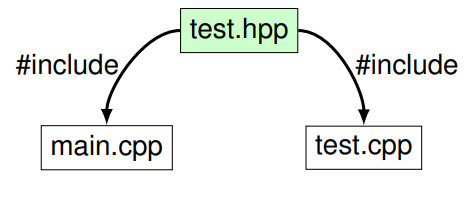
\includegraphics[scale = 0.6]{Capitoli/Compilatore/Esempi/esempioMultiplaInc.png}
\end{center}
\textbf{Come possiamo risolvere?} Basterà inserire nel file Header un \textbf{"flag"} che ci indichi se quel file è stato già inserito o meno.
\lstinputlisting{Capitoli/Compilatore/Esempi/testhppflag.txt}
quando viene incluso il file \code{test.hpp} prima di essere inserito nel file controllerà se \code{TEST\_HPP} non sia già stata dichiarata, nel caso in cui lo fosse non sarà incluso nulla.

\subsubsection{Sudivisone File Haeder File}
\begin{itemize}
 \item gli Header contiene \textbf{l'interfaccia} di tutto il contenuto del file sorgente corrispondente 
 \item Ogni file sorgente contiene un \code{\#include} per l’header
    corrispondente e poi eventuali altri header per tutto ciò che
    utilizza e la cui implementazione è data in altri file
 \item creare un file header \code{.hpp} per ogni file sorgente \code{.cpp}
\end{itemize}


\subsection{Fasi compilazione}

In questa fase abbiamo 4 fasi che restituiscono i seguenti file(Nome file "\code{primo.cpp}"):
\begin{itemize}
    \item \textbf{primo.i:} output Preprocessing
    \item \textbf{primo.s:} output fase di Compiling
    \item \textbf{primo.o:} output assembly
    \item \textbf{a.out:} output della fase di linking
\end{itemize}

\subsubsection{Preprocessing stage}
in questa fase succederà:
\begin{itemize}
    
    \item rimozione commenti
    \item saranno esegui le macro (es. \code{\#define}) , verranno sostituite al interno del programma 
    \item i file saranno inclusi attraverso \code{\#include}
    verranno inseriti le posizioni precisi dei file inclusi 
    esegue tutte le azioni precedute dal \code{\#}
\end{itemize}

\subsubsection{Compiling stage}
in questa fase viene creato il codice assembly. Ogni macchina ha la propria architettura e il proprio 
funzionamento. Per colpa di quest'ultima il codice assembly varia da processore a processore. Per 
questo ogni volta che il programma viene compilato sarà trasformato prima in assembly.

\newpage

\subsubsection{Assembly stage}
\begin{itemize}
    \item il \textbf{codice assembly} viene convertito in linguaggio macchina
    \item il file risultato è chiamato file oggetto
    \item \textbf{non risolve} chiamate a funzione.
    \item il file output non sarà visibile con normali tool di testo perché verranno codificati in \code{ASCII}
    \item il file oggetto \code{.o} può essere generato tramite il flag -c: \newline  \code{gcc -c primo.c} . questo comando farà tutti le fasi tranne il linking cosi non generando l'eseguibile.
\end{itemize}

\subsubsection{Linking stage}
    \begin{itemize}
        \item vengono risolte le \textbf{chiamate a funzione}. verranno uniti tutti i file oggetti fra di loro
        \item viene creato l’eseguibile
    \end{itemize}
\newpage
\section{Tipi di dati}
\subsection{Tipi fondamentali}
In \code{C++} abbiamo dei \textbf{tipi fondamentali}, che sono implementati di base dal linguaggio. Si chiamano \textbf{Built-in(integrati)}\newline
questi tipi sono: 
\begin{itemize}
    \item \textbf{\textcolor{blue}{Built-in (Integrati)}:}
        \begin{itemize}
            \item \code{\textbf{Boolean}}
            \item \code{\textbf{char}}
            \item \code{\textbf{int} , long int, long long int...}
            \item \code{float , \textbf{double}, long double}
            \item \textbf{void}
            \item \textbf{Puntatori(es: \code{int*})}, \textbf{Array} e \textbf{Riferimenti(\code{double\&})}
        \end{itemize}
    \item \textbf{\textcolor{blue}{User-defined}:}
        \begin{itemize}
            \item enum
            \item \textbf{classes}
            \item \textbf{tipi introdotti dalle librerie standard}
        \end{itemize}
\end{itemize}
Un \textbf{'\code{tipo}'} serve per definire il \textbf{dominio} dei valori che può assumere quel elemento. Il \textbf{'\code{tipo}'} serve anche per definire l'insieme di \textbf{operazioni} che si possono essere fate su quel tipo. \newline\newline
poi intendiamo come \textbf{letterale} tutti i valori inseriti direttamente nel codice
\lstinputlisting{Capitoli/Tipi di dato/Esempi/Esletterali.txt}

\newpage
\subsubsection{Sizeof()}
Il \code{Sizeof()} permette di controllare lo spazio che occupa un determinato tipo o variabile. Il peso dei tipi va in base all'implementazione del programmatore. Quindi il programmatore può modificare le grandezze di default.
questo può comportare dei vantaggi e dei svantaggi.\newline\newline
 \textbf{\textcolor{blue}{Vantaggi:}}
\begin{itemize}
    \item Utilizzando grandezze personalizzate posso sfruttare a meglio il mio hardware(memoria)\newline
\end{itemize}
\textbf{\textcolor{blue}{Svantaggi:}}
\begin{itemize}
    \item Il codice diventa meno portatile poiché diventerebbe più specifico per un certo hardware(meno portatile)
    \item rischio che con le versioni future del compilatore non potrebbe funzionare poiché si sono modificati valori di default
\end{itemize}

Quindi dobbiamo modificare questi valori solo quando è veramente necessario poiché a noi ci interessa la portabilità del codice

\subsection{Inizializzazioni}
\hypertarget{init}{}
Possiamo inizializzare una variabile in 4 modi:

\begin{enumerate}
    \item Graffe(list initialization): \code{int a1 \{15\}};
    \item Uguale + graffe: \code{int a2 = \{15\};}
    \item Uguale: \code{ int a3 = 15;}
    \item Tonde:  \code{int a4(15);}
\end{enumerate}
\textbf{\textcolor{blue}{Cosa utilizzare?}}
\begin{itemize}
    \item La prima forma è \textbf{PREFERIBILE} poiché controlla che varie conversioni non perdano informazioni.
    \item Se non viene inserito nessun valore viene inizializzato a un valore di default, questo metodo di inizializzazione e più leggibile e permette meno errori.
    \lstinputlisting{Capitoli/Tipi di dato/Esempi/InParentesigraffeEs.txt}
\end{itemize}
Possiamo inizializzare anche una lista di elementi:
\lstinputlisting{Capitoli/Tipi di dato/Esempi/vettoreIn.txt}

\subsection{Tipo Booleano}
Il tipo booleano può essere solo due valori \textcolor{blue}{\code{True}} o \textcolor{blue}{\code{False}}.\newline Possiamo subito dire che: 
\begin{itemize}
    \item Un qualsiasi valore intero diverso da zero è convertito in booleano come  \textcolor{blue}{\code{True}}, altrimenti un valore uguale a zero come  \textcolor{blue}{\code{False}}
    \lstinputlisting{Capitoli/Tipi di dato/Esempi/EsempioconversioneBool.txt}
    \item Un puntatore può essere convertito \code{True} se punta a qualcosa , altrimenti se non punta a nulla(\code{nullptr}) a \code{false}
\end{itemize}

\subsection{Tipo carattere}
Esistono vari tipi di caratteri (come i latini o gli ideogrammi cinesi ecc.) ognuno di essi ha la sua propia codifica.\newline\newline
Ovviamente non esiste solo il tipo \code{char}, Esistono numerosi tipi che supportano anche diversi tipi di codifica. nella maggior parte dei casi basta il \code{char} con i suoi \code{8 bits}. \newline\newline
Il \code{char} supporta la codifica ASCII ed è in grado di immagazzinare un solo carattere (1 Byte). \newline\newline
Esistono anche dei caratteri speciali che utilizzano il carattere " \textbackslash " come "\textbackslash n".
\newpage
\subsection{Tipo Intero}
Abbiamo diversi tipi di intero:
\begin{itemize}
    \item Con il segno(\code{unsigned})
    \item Diverse dimensioni(\code{int , short int , long int ecc.})
\end{itemize}
\begin{itemize}
    \item utilizzare \code{unsigned} per risparmiare \code{1 bit} non ha senso, è quasi in rilevante in vasta scala.
    \item \textbf{letterali} sono interi e tutti espressi in decimale , esadecimale , ottale(es: base 10(1), base 16(0x1) , base 8(01))
    \item Il tipo di ogni letterale è deciso dal suo suffisso, se c’è (ad
    esempio: u o U per \code{usigned}, l o L for \code{long}, ll o LL for \code{long long}) e dal tipo di lunghezza minima che ne contiene il
    valore.

\end{itemize}


\subsection{Tipo virgola mobile (floating point)}
\begin{itemize}
    \item \code{double} è il \textbf{default}. Quindi il tipo base per esprimere numeri con la virgola.
    \item I Sono letterali validi: 1.23, .23, -2.3, 0.23, 1., 1.0, 1.2e10,
    1.23e-15 (niente spazi attorno alla e)
    \item Suffisso f se voglio che sia un \code{float (2.0f)}
    \item Suffisso L per \code{long double}.
\end{itemize}

\subsection{Tipo void}
\begin{itemize}
    \item  Non possono esistere oggetti di tipo void.
    
    \item Si usa solo in due casi:
        \begin{enumerate}
            \item Per indicare che una funzione non restituisce nulla;
            \item Per indicare il tipo di un puntatore ad un oggetto di tipo
            sconosciuto
        \end{enumerate}
\end{itemize}
\newpage
\subsection{Tipo costante}
\textbf{\textcolor{blue}{\code{const}}}: “Prometto di non cambiare questo valore” e il compilatore controlla che sia proprio così. \newline
\textbf{\textcolor{blue}{\code{constexpr }}}: “Da valutare a tempo di compilazione”.
Possono essere \code{constexpr} anche funzioni, ma solo se
molto semplici (solo un’istruzione di \code{return})\newline
Distinzione sottile, che per il momento potete non
considerare

\subsection{Tipo punatore e riferimento}
\begin{itemize}
    \item Possiamo accedere a una variabile nei seguenti modi:
    \begin{itemize}
        \item usando il nome
        \item dal suo indirizzo di memoria, tenendo conto del tipo della
        variabile
        \item dal suo riferimento
    \end{itemize}
    \item Puntatori e riferimenti servono esattamente a questo, in
    due modi leggermente diversi.
\end{itemize}
 Esempio di puntatore:
 \lstinputlisting{Capitoli/Tipi di dato/Esempi/EsPtr.txt}
 \begin{center}
     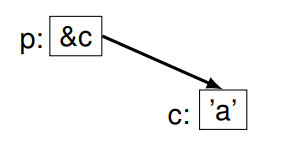
\includegraphics[scale = 0.6]{Capitoli/Tipi di dato/Esempi/ptr.png}
 \end{center}
 \begin{itemize}
     \item \code{c2} assume il valore puntato da \code{p}, nel senso che \code{c2} assume il valore memorizzato all’indirizzo contenuto in \code{p}
    \item quindi: la memoria viene letta sapendo il tipo della
    variabile, altrimenti sarebbe impossibile.
    \item L’oggetto puntato da \code{p} è \code{c}, il cui valore è \code{’a’}
    \item in conclusione: \code{c2} assume il valore del letterale \code{’a’}
 \end{itemize}
Quando accediamo a un valore puntato da un puntatore(quindi trmite l'Indirizzo contenuto nel puntatore) stiamo effettuando la differenziazione tramite l'operatore unario \textcolor{blue}{\code{*}}.\newline\newline
I puntatori hanno una aritmetica chiamata \textbf{aritmetica dei puntatori} che utilizza l'indirizzamento della memoria. Ci permette di lavorare sugli indirizzi facendo delle operazioni(es: sommare un valore a un indirizzo) su questi indirizzi. Questa indirizzazione avviene tramite \textbf{bytes}.\newline\newline
Quindi il più piccolo oggetto che può venir allocato e
indirizzato indipendentemente è il \code{char}, che corrisponde
ad un byte. infatti il \code{bool} occupa almeno tanta memoria quanto un \code{char}.\newline\newline
Ottimo se ho bisogno di implementare applicazioni che
scendano a quel livello di dettaglio (ad esempio, un
sistema operativo) \newline Se invece voglio fare una buona applicazione portabile,
meglio non usare queste operazioni di basso livello.\newline\newline\newline
\textbf{Per trasformare} un qualsiasi tipo \code{X} nel
corrispondente puntatore a \code{X} dobbiamo aggiungere al tipo
il suffisso \code{*}\newline\newline
\lstinputlisting{Capitoli/Tipi di dato/Esempi/EsPtr2.txt}
\textbf{Invece per le funzioni:}
\lstinputlisting{Capitoli/Tipi di dato/Esempi/EsPtr3Funz.txt}
\newpage 
\subsubsection{Puntatori a void}
\begin{itemize}
    \item Se dichiariamo una variabile di tipo \code{void*}, le possiamo
    assegnare un puntatore ad un qualsiasi tipo di oggetto.
    \item Possiamo considerarlo un \textbf{puntatore ad un oggetto di
    tipo sconosciuto}
    \item \textbf{Però} non può essere né un puntatore a funzione né un
    puntatore a un membro di una classe (inclusi i membri
    funzione o metodi)
    \item Se ho due variabili di tipo \code{void*}, posso:
    \begin{itemize}
        \item assegnare il valore dell’una all’altra
        \item confrontarle (sia eguaglianza che diseguaglianza)
        \item posso convertirle \textbf{esplicitamente} ad un altro tipo \end{itemize}
    \item Qualsiasi altra operazione può essere \textbf{pericolosa} e quindi
    va evitata: dà \textbf{errore} a tempo di compilazione
    \item Per usare un \code{void*} dobbiamo convertirlo esplicitamente
    ad un puntatore di un dato tipo
    \lstinputlisting{Capitoli/Tipi di dato/Esempi/EsPtrVoid.txt}
\end{itemize}
\code{int* pi2 = static\_cast<int*>(pv);}\newline dove \code{static\_cast<int*>} è un cast statico , questo cast aviene durante la compilazione e non durate il run-time
\begin{itemize}
    \item In genere, usare un puntatore ad un tipo \code{X1} per puntare ad  un oggetto di tipo \code{X2} è pericoloso(es: Il codi qui sopra). quindi usare il "cast" potrebbe creare problemi
    \item Pensiamo ad esempio che la dimensione di un oggetto
    può dipendere dall’implementazione . . .
    \item Cerchiamo quindi di usare questo operatore il meno
    possibile
    \item Il puntatore \code{void*} si usa per operazioni a basso livello sulla memoria
    \item In questi casi, gli usi più diffusi di \code{void*} sono:
    \begin{itemize}
        \item voglio passare un parametro ad una funzione senza fare
        ipotesi sul tipo dell’oggetto puntato
        \item la funzione deve tornare un puntatore ma senza fare ipotesi sul tipo dell’oggetto puntato
    \end{itemize}
    
    \item Se l’operazione è a più alto livello, meglio utilizzare
    soluzioni basate su un progetto orientato agli oggetti

\end{itemize}

\subsubsection{nullptr}
Letterale che rappresenta il \textbf{puntatore nullo}, ovvero il
puntatore che non punta a nessun oggetto
I Può venir assegnato a qualsiasi tipo di puntatore, ma non
agli altri tipi \textcolor{blue}{built-in}:
\lstinputlisting{Capitoli/Tipi di dato/Esempi/Esnullptr.txt}
 Un unico \code{nullptr} per qualsiasi tipo di puntatore
 \begin{itemize}
    \item Nessun oggetto può venir allocato all’indirizzo 0 (ovvero il
    pattern con tutti i bit a zero), quindi una volta si usava
    l’intero 0 al posto del puntatore nullo
    \item Addirittura si definiva una macro \code{NULL} per rappresentare il
    puntatore \code{null}
    \item Tuttavia
    \begin{itemize}
        \item la definizione di \code{NULL} dipende dall’implementazione (ad esempio, può essere 0 o 0L)
        \item la definizione usata in \code{C} (\code{(void*)0}) è illegale in \code{C++}
    \end{itemize}
    \item Conclusione: usate \code{nullptr}!

 \end{itemize}
\newpage

 \subsection{Array}
 \begin{itemize}
    \item Un array è una raccolta di dati di tipi omogenei fra di loro.
    \item Un array di Tipo \textcolor{blue}{\textbf{\code{X}}} deve essere indicato nel seguente modo se è definito in modo statico \textcolor{blue}{\textbf{\code{X NomeArray[size]}}}.
    l'indice va da \code{0} (index 0) fino a \code{size-1}(index -1)
     \lstinputlisting{Capitoli/Tipi di dato/Esempi/EsArray.txt}
    \item Possiamo usare l'operatore \textcolor{blue}{\code{[]}} per accedere oppure l'operatore unario \textcolor{blue}{\code{*}} (preferibile \textcolor{blue}{\code{[]}} poiché \textcolor{blue}{\code{*}} lavora troppo a basso livello)
    \item andare oltre alla lunghezza del array ha un comportamento indefinito e disastroso poiché non si sa cosa c'è dopo.
    \item quando inizializziamo un array la grandezza (\textcolor{blue}{\code{size}}) deve essere ben definita cioè un letterale. altrimenti il comportamento è indefinito. 
    \item possiamo invece usare il \textbf{\textcolor{blue}{\code{Vector}}} all'interno della standard library. a differenza del array conserverà la sua grandezza e quindi può essere definita come una variabile.
    \lstinputlisting{Capitoli/Tipi di dato/Esempi/EsArray2.txt}
 \end{itemize}
\textbf{\textcolor{blue}{Limitazioni Array built-in:}}
\begin{itemize}
    \item Si tratta di una struttura inerentemente di \textbf{basso livello}, da usarsi essenzialmente per costruire strutture di più \textbf{alto
    livello}, quali le strutture \textbf{vector} e \textbf{array} della libreria standard.
    \begin{itemize}
        \item  Non è possibile assegnare un \textbf{array} ad un altro \textbf{array}. Questo a meno che \textbf{l'array} destinazione non sia un puntatore a il tipo del \textbf{array} che dovrà essere assegnato.
        \lstinputlisting{Capitoli/Tipi di dato/Esempi/EsArray3.txt}
        \item  Come conseguenza, non è possibile passare un \textbf{array} ad
        una funzione per valore(altrimenti  si dovrebbe copiare l'intero \textbf{array}).
        \item  Il nome di un \textbf{array} viene implicitamente convertito ad un puntatore al suo primo elemento in molti contesti (poi
        vediamo meglio)
    \end{itemize}
    
    \item  Uno degli \textbf{array} più utilizzati è \textbf{l’array} di \code{char} terminato dal \code{char \textbackslash0}: una stringa in stile C: conservata per compatibilità con librerie già esistenti.

\end{itemize}


\subsubsection{Inizializzazione Array}
Possiamo inizializzare un Array in diversi modi:
\lstinputlisting{Capitoli/Tipi di dato/Esempi/InitArrayes.txt}
\begin{itemize}
    \item Nel caso in cui specifichiamo la dimensione e non inseriremo abbastanza elementi durante la inizializzazione allora saranno impostati a zero.
    \item Se non definiamo il numero di elementi che conterrà un array ma definiamo qual'è elemento ci dovrà essere allora il compilatore capirà da solo quanto spazzino allocare.
\end{itemize}
\subsubsection{Letterali stringa}
Un letterale stringa è un tipo costante (\code{const char}). Ogni letterale finisce con \code{'\textbackslash 0'}. \newline
Ogni carattere occupa \code{1 byte} quindi un letterale con 5 caratteri sarà un \newline\code{const char[5]}
\begin{itemize}
    \item \textbf{letterali stringa sono costanti, quindi immutabili}.
    \item  Se vogliamo usarla come inizializzazione e poi modificarla,
    dobbiamo usare l’array di caratteri (non costante):
    \lstinputlisting{Capitoli/Tipi di dato/Esempi/EsletString.txt}
    \item letterali stringa sono \textbf{allocati staticamente}, quindi possono essere restituiti da funzioni in modo sicuro. Poiché dopo alla chiamata di funzione la stringa è allocata in modo statico non sarà persa.
    
    \lstinputlisting{Capitoli/Tipi di dato/Esempi/EsritString.txt}
    \item Il codice viene \textbf{ottimizzato}, quindi in alcuni casi può
    succedere che due letterali stringa identici non vengano
    duplicati. quindi viene usato lo stesso letterale.
    \item Questo significa che non possiamo ipotizzare con certezza
    cosa succede.
    \lstinputlisting{Capitoli/Tipi di dato/Esempi/EsotString.txt}
    \item L’espressione \textcolor{blue}{\code{p==q}} confronta gli indirizzi, cioè i valori
    dei puntatori e non degli oggetti puntati.
    \item La lista vuota è \code{""}, ha tipo \code{const char[1]} e contiene il
    solo carattere \code{’\textbackslash 0’}.
    \item Per rappresentare i caratteri non grafici all’interno di una
    stringa possiamo utilizzare il \code{\textbackslash}:\newline
    \code{cout << "beep at end of message\textbackslash a\textbackslash n";}\newline
    \item Un problema possono essere le stringhe contenenti il
    carattere nullo
    \begin{itemize}
        \item  Sono perfettamente legali.
        \item La maggior parte dei programmi considererà solo la parte
        prima del primo carattere nullo: \code{Jens\textbackslash000Munk} verrà considerato come \code{"Jens"}.
        
    \end{itemize}
    \item  Il carattere di \textbf{newline} non può essere incluso in una
    stringa: una stringa non può stare su più righe. Devo
    invece usare \code{’\textbackslash n’}
    \item Se una stringa è troppo lunga può essere spezzata
    \lstinputlisting{Capitoli/Tipi di dato/Esempi/SpezString.txt}
\end{itemize}
\newpage
\subsubsection{Array come puntatore}
\begin{itemize}
    \item Legame stretto tra array e puntatori: il nome di un array
    può venir utilizzato come \textbf{puntatore al suo primo elemento}.
    \lstinputlisting{Capitoli/Tipi di dato/Esempi/EsPtrArray.txt}
    \begin{center}
        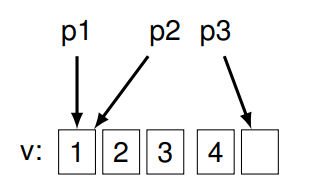
\includegraphics[scale = 0.6]{Capitoli/Tipi di dato/Esempi/EsPtrArray.png}
    \end{center}
    \item \textbf{Puntare} ad un elemento immediatamente successivo alla
    fine dell’array non dà errore, purché non si legga o scriva.
    \item Quando passiamo un \code{array} come parametro non ci sarà modo di passare una copia. sarà sempre passato il \textbf{riferimento} , questa conversione implicita da \textcolor{blue}{\code{array}} a  \textcolor{blue}{\code{puntatore}} farà perdere la grandezza del \code{array}.
    quindi non ci sarà modo di evitare questa conversione implicita.
    \lstinputlisting{Capitoli/Tipi di      dato/Esempi/EsempiArrayDopoSize.txt}
\end{itemize}
\newpage
\subsubsection{Navigazioni degli Array}
Abbiamo due modi per navigare in un array:
\begin{itemize}
    \item Utilizzare l'operatore \textcolor{blue}{\code{*}}. quindi sommare al indirizzo del \code{array} \textbf{l'indice} che vogliamo raggiungere e poi fare la Dereferenziazione per ottenere il contenuto.
    \item Utilizzare le \textbf{parenesi quadrate} con al interno l'indice
    \item \textbf{nessuna delle due e più efficiente del altra}, per una questione di leggibilità e meglio con le parentesi quadrate.
    \lstinputlisting{Capitoli/Tipi di dato/Esempi/NavigazioneArray.txt}
\end{itemize}

\subsubsection{Array Multidimensionali e Array come argomento di funzione}
\begin{itemize}
    \item Gli array multidimensionali sono rappresentati come array
    di array
    \item I Esempio 3x5:
    \lstinputlisting{Capitoli/Tipi di dato/Esempi/Matrix.txt}
    \item  Come per gli \code{array} ad una sola dimensione, le
    dimensioni non sono memorizzate in alcun modo nella
    struttura dati \code{array}
    \item Un array non può venir passato ad una funzione per
    valore, ma con un puntatore al suo primo elemento
    \lstinputlisting{Capitoli/Tipi di dato/Esempi/PassaggioArrayPar.txt}
\end{itemize}

\subsection{Riferimenti}
\begin{itemize}
    \item  \textbf{Un riferimento} (reference) può essere visto come un nome
    alternativo per un oggetto, un alias.
    \item \textcolor{blue}{\textbf{Analogamente ai puntatori:}}
    \begin{itemize}
        \item è un alias per un oggetto
        \item è implementato per conservare l’indirizzo di un oggetto
        \item non richiede maggiori risorse computazionali
    \end{itemize}

    \item \textcolor{blue}{\textbf{Diversamente dai puntatori, il riferimento:}}
    \begin{itemize}
        \item la sintassi è la stessa che avrei col nome dell'oggetto
        \item si riferisce sempre all'oggetto con cui è stata inizializzata
        \item \textbf{non esiste un “riferimento null”} da controllare: ogni
        riferimento si riferisce ad un oggetto
        \lstinputlisting{Capitoli/Tipi di dato/Esempi/EsempioReferance.txt}
    \end{itemize}
    \item Tra i \textbf{vantaggi} dei puntatori c’è quello di poter passare ad
    esempio ad una funzione una grande quantità di dati a
    basso costo.
    \item Però un puntatore ha una sintassi un po’ pesante . . .
    \item e può cambiare valore nel tempo, Invece il \textbf{riferimento} si riferirà \textbf{\textcolor{blue}{SEMPRE}} al oggetto a cui è stato inizializzato
    \item Inoltre bisogna sempre gestire la possibilità che il
    puntatore non stia puntando a nulla \textbf{(nullptr)}.
    \item Coi riferimenti non ho questi problemi.

\end{itemize}



\section{Allocazione in memoria}

La vita di un oggetto è determinata dal suo \textbf{scope}(è un blocco di codice tra parentesi graffe).\newline\newline
A volte ci occorre creare un oggetto che venga \textbf{allocato} nella free memory(heap) e venga \textbf{deallocato} solo quando noi lo vogliamo.\newline\newline
Quindi una variabile che vive indipendente dallo \textbf{scope}
\begin{tcolorbox}[width=\linewidth, boxsep=6pt]
Queste sono le parole \textbf{\code{\textcolor{blue}{chiavi}}} per lavorare sulla \textbf{free memory}:
\lstinputlisting{Capitoli/Allocazione Memoria/Esempi/Key_De_Allocazione.txt}
\end{tcolorbox}

\newpage

\subsection{Key New}
\begin{itemize}
    \item \textcolor{blue}{\code{New}} crea un oggetto sullo \code{heap}
    \item Se la memoria è insufficiente lancerà un eccezione 
    \code{bad\_alloc}
    \item in caso di buona allocazione sarà restituito un \textbf{puntatore} alla locazione di memoria allocata
    \lstinputlisting{Capitoli/Allocazione Memoria/Esempi/EsAllocazioni.txt}
    \item Gli oggetto allocati con \code{\textbf{new}} rimarranno allocati in memoria finché non verranno Deallocati \textbf{esplicitamente}
    \lstinputlisting{Capitoli/Allocazione Memoria/Esempi/EsDeallocazione.txt}
    \item \code{new} un oggetto verrà allocato con la parola \code{new} e sarà richiamato il costruttore della classe(avviene di default anche se non specificato)
\end{itemize}

\subsection{Key Delete}
\begin{itemize}
    \item \textcolor{blue}{\code{delete}} è un operatore che può essere utilizzato solo sui \textbf{puntatori} ritornati da \code{new} oppure su puntatori a null(\code{nullptr})
    \item L'Applicazione di \code{delete} su \code{nullptr} non avrà nessun effetto
    \item Se un oggetto è stato creato con \code{new} esso esiste fino a
    quando non viene esplicitamente distrutto con \code{delete}.
    \item Solo dopo aver usato \code{delete} a quel punto lo spazio in memoria occupato dall’oggetto può venir riutilizzato.
    \item Se \code{delete} viene utilizzata su una \textbf{classe} e in questa \textbf{classe} sarà definito un \textbf{distruttore} allora prima che la memoria venga liberata verrà eseguito il \textbf{distruttore}.
\end{itemize}
\newpage
\subsection{Key Delete[]}
\begin{itemize}
    \item Per liberare lo spazio allocato da una \textcolor{blue}{\code{new}}, sia \textcolor{blue}{\code{delete}} che \textcolor{blue}{\code{delete[]}} devono conoscere la dimensione dell’oggetto
    allocato.
    \item A \textcolor{blue}{\code{delete}} basta conoscere il tipo dell’oggetto puntato(facilmente reperibile).
    \item Ma \textcolor{blue}{\code{delete[]}} deve conoscere anche il numero di
    oggetti puntati.
    \item Quando viene allocata memoria sullo \textbf{heap}, la \textcolor{blue}{\code{new []}} tiene traccia di quanta memoria/numero di elementi
    allocata/i,
    \item di solito salvando l’informazione in un segmento che
    precede immediatamente la memoria allocata.
    \item Ne consegue che un oggetto array allocato mediante
    l’implementazione standard di \textcolor{blue}{\code{new}} occuperà uno spazio
    leggermente superiore del corrispondente statico.
    \item Quanto meno, infatti, lo spazio necessario a contenere la
    dimensione dell’oggetto.
    \begin{tcolorbox}[width=\linewidth, boxsep=6pt]
    \textcolor{red}{\textbf{NB:}} \textcolor{blue}{\textbf{\code{sizeof}}} restituisce solo la grandezza di un \textbf{tipo} specificato \textbf{NON} della memoria fisicamente allocata di una certa istanza. \newline\newline Quindi il calcolo della grandezza di un  tipo di dato avviene alla \textbf{\textcolor{blue}{\code{Compilazione}}} invece il numero di elementi di può sapere solo al tempo di \textbf{\textcolor{blue}{\code{Esecuzione}}}.
    \end{tcolorbox}
    \item Questo vale solo per l’allocazione degli array: in tutti gli
    altri casi viene usato il tipo del puntatore.
\end{itemize}

\subsection{Gestione memoria}
I principali problemi della memoria \textbf{Libera}(Free memory) è:
\begin{itemize}
    \item \textbf{\textcolor{blue}{Ogetti abbandonati(leaked objects)}}: Allocare uno spazio di memoria con \textcolor{blue}{\code{new}} e poi dimenticarsi di usare \textcolor{blue}{\code{delete}} quando non serve più
    \item \textbf{\textcolor{blue}{Cancellazione prematura(Premature deletion)}}: Quando cancelliamo una locazione(\code{delete}) di memoria in modo prematuro. quindi dealloco una porzione di memoria e poi in un altra parte del codice ho un puntatore a questa locazione ormai libera, quindi accendendo a una locazione liberata il comportamento è indefinito.
    \item \textbf{\textcolor{blue}{Doppia cancellazione(Double deletion)}}: Un oggetto deallocato due volte poiché si chiama due volte il suo distruttore.
    
\end{itemize}

\begin{tcolorbox}[width=15cm, boxsep=10pt]
    \textbf{\textcolor{red}{Esempio Cancellazione prematura:}}
    \lstinputlisting{Capitoli/Allocazione Memoria/Esempi/EsbadFreeMem.txt}
    \textcolor{red}{\textbf{NB:}} Perché \textcolor{blue}{\code{p3}} punterà alla stessa locazione di \textcolor{blue}{\code{p2}} ? Questo perché la \textbf{memoria} per allocare oggetti del nostro programma è \textbf{ben precisa}. Si inizia ad \textbf{allocare} dal primo \textbf{indirizzo} fino al ultimo della memoria dedicata al nostro programma. In questo esempio abbiamo allocato un \textcolor{blue}{\code{int}}(che occupa i primi \code{8 bytes}) e subito dopo lo \textbf{de-allochiamo}. quando \textbf{allochiamo} una nuova porzione di memoria cerchiamo uno spazio libero per l'allocazione(che nel nostro deve poter contenere un \textcolor{blue}{\code{char}}) , essendo la \textbf{memoria vuota} lo inserirà a partire dal primo indirizzo delle memoria dedicata al programma. Essendo che \textbf{punterà} proprio a quel indirizzo quando andremo a assegnare un \code{int(999)} sarà valutato come un \textcolor{blue}{\code{char}} ed uscirà \code{þ}(Simbolo associato al codice ASCII).
\end{tcolorbox}
\subsubsection{Problemi: Doppia cancellazione}
\begin{itemize}
    \item Il problema nasce dal fatto che tipicamente il gestore delle
    risorse non è in grado di tenere traccia di quale parte di codice è proprietaria di una risorsa. quindi se faccio una doppia cancellazione io non so quella locazione di memoria effettivamente apparteneva originariamente apparteneva a qualche altra funzione
    \item Quindi il risultato di un doppio \textcolor{blue}{\code{delete}} non è prevedibile
    \lstinputlisting{Capitoli/Allocazione Memoria/Esempi/DoppiaCanc.txt}
    \item Tra il primo e il secondo \textcolor{blue}{delete[]} la memoria può essere stata riutilizzata
\end{itemize}

\subsection{Buone norme d'utilizzo}
\begin{itemize}
    \item Evitiamo di mettere oggetti sullo free store a meno che non
    sia strettamente necessario: meglio usare uno scope il più
    ristretto possibile
    \item Quando un oggetto viene costruito sullo free store, meglio
    inserirlo all’interno di un \textbf{gestore di oggetti} (handle) che
    preveda un distruttore
    \item Come regola pratica: usiamo \textcolor{blue}{\code{new}} dove c’è un costruttore e
    \textcolor{blue}{\code{delete}} dove c’è un distruttore
\end{itemize}

\subsection{Prestazioni}
\begin{itemize}
    \item Una gestione poco attenta dello heap (alternanza di \code{new} e
    \code{delete}) può portare alla sua \textbf{frammentazione}: la
    formazione di buchi nella memoria disponibile.
    \item Questi buchi sono troppo piccoli per poter essere utilizzati
    per allocare nuovi oggetti.
    \item L’effetto è che la memoria che resta disponibile è molto
    meno di quello che ci si aspettava.
    \item Ne consegue anche \textbf{l’aumento dei tempi} di esecuzioni di
    nuovi \code{new}: diventa sempre più difficile andare a cercare
    dove poter mettere il nuovo oggetto.
    \item Cerchiamo di capire come funziona questo meccanismo
    per cercare di prevenirlo
\end{itemize}
\begin{tcolorbox}[width=15cm, boxsep=10pt]
    \lstinputlisting{Capitoli/Allocazione Memoria/Esempi/EsFramenttazione.txt}
    
\end{tcolorbox}
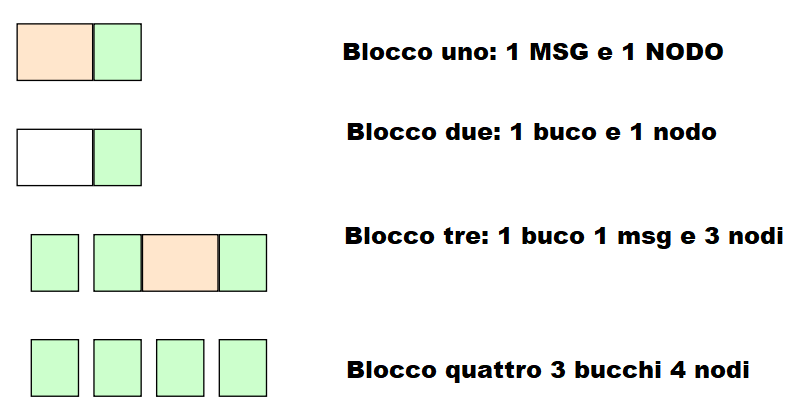
\includegraphics[scale = 0.4]{Capitoli/Allocazione Memoria/Esempi/Blocchi.png}\newline
\begin{itemize}
    \item In questo esempio si vede benissimo che ogni volta che cancello un \  \newline\textcolor{orange}{messaggio} e alloco un nodo si crea un buco poiché il \textcolor{green}{nodo} non è grande quanto la memoria libera creando un buco che non può essere riempito da \newline\textcolor{orange}{messaggio}. reiterando questo blocco di codice avremo sempre piu buchi non utilizzabili
\end{itemize}

\subsection{Soluzioni alla framenttazione}
\begin{itemize}
    \item Due alternative:
    \begin{itemize}
        \item  Un \textbf{garbage collector} per tappare i buchi
        \item  Il programmatore evita di crearli
    \end{itemize}
    \item I puntatori rendono difficile creare un \textbf{garbage collector}
        \begin{itemize}
            \item poiché è difficile spostare le locazioni di memoria al interno della memoria rispetto ad altri linguaggi come \textbf{java} dove si posso spostare gli oggetti al interno della memoria più facilmente 
        \end{itemize}
    \item Come possiamo evitare la formazione dei buchi?
    \item A volte basta riorganizzare la chiamata alle \code{new} e \code{delete}
    \item Ma non è una soluzione generale
    \item \textbf{Prevenire:} evitare usi del free store che provocano
    frammentazione
    \item \textbf{Prima idea:} evitiamo l’uso del \code{delete}, almeno non
    rallentiamo nuovi \code{new}, almeno nella maggior parte delle
    implementazioni, anche se non è garantito dallo standard.
    \item \textbf{Seconda idea:} allochiamo tutta la memoria (statica e
    globale) all’inizio del programma e poi la usiamo.\newline\newline
    \textcolor{blue}{\textbf{Svantaggi:}} struttura del programma non ottimale e uso di
    dati globali da evitare.
\item Due \textbf{strutture} dati possono \textbf{aiutarci} in questo:
    \begin{itemize}
        \item  \textcolor{blue}{\textbf{Stack}} : visto che si allunga e si accorcia solo da una
        parte non può causare frammentazione
        \item \textcolor{blue}{\textbf{Pool}} : una raccolta di oggetti della stessa
        dimensione. Essendo della stessa
        dimensione, non può esserci frammentazione.
    \end{itemize}
    \item Con entrambe queste soluzioni, sia \textbf{l’allocazione} che la
    \textbf{deallocazione} hanno tempi prevedibili e veloci.
    Se non si gestisce la frammentazione potremo avere tempi lunghi di allocazione e non prevedibili
\end{itemize}

\section{Tipi definiti dal utente}
Abbiamo visto finora dei tipi \textbf{built-in(integrati)} che sono di molto \textbf{basso livello} è sono difficili per un programmatore gestirli e creare applicazioni di alto livello.\newline
per questo \code{C++} mette a disposizione \textbf{i meccanismi d'astrazione} con cui so costruiscono strutture di \textbf{alto livello}. Queste strutture vengono chiamate \textbf{\textcolor{blue}{tipi definiti dai utenti}(user-defined types)}\newline \newline
\textbf{Questi tipi definiti dai utenti sono:} 
\begin{itemize}
    \item Classi
    \item Enumeratori
    \item Struct
\end{itemize}

\subsection{Esempi di user-defined types}
Un Esempio di tipo di dato definito dal utente è un vector:
\lstinputlisting{Capitoli/Tipi definiti dai utenti/esempi/vector.txt}
Questa è la prima versione di una migliore gestione del vettore. \newline\newline
\textbf{Abbiamo:}
\begin{itemize}
    \item \textbf{Primo blocco} definiamo un tipo vector
    \item \textbf{Secondo blocco} creiamo una variabile di tipo vector
    \item \textbf{Terzo blocco} definiamo una funzione per l'inizializzazione
    \item Allochiamo l’array elem sullo heap.
    \item Si noti che il primo argomento (\textcolor{blue}{\code{Vector\& v}}) è passato per
    riferimento, in modo da poterlo modificare
\end{itemize}
\begin{tcolorbox}[width=15cm, boxsep=10pt]
    Un utilizzo di questo \textbf{vector} può essere il seguente:
    \lstinputlisting{Capitoli/Tipi definiti dai utenti/esempi/utilizzovector.txt}
    \textcolor{blue}{\textbf{NB}:} in questo caso Il programmatore deve conoscere le strutture interne dell'oggetto
\end{tcolorbox}
\newpage
\subsection{Classi}
Una \textcolor{blue}{\textbf{classe}} è un insieme di:
\begin{itemize}
    \item Attributi
    \item Metodi
\end{itemize}
\textbf{L'interfaccia} della classe è data dalla \textbf{visibilità} dei suoi metodi e attributi(quindi da quelli \textbf{pubblici}). abbiamo anche dei attributi o metodi \textbf{privati} che sono visibili solo al interno della classe.
\begin{tcolorbox}[width=15cm, boxsep=10pt]
    \lstinputlisting{Capitoli/Tipi definiti dai utenti/esempi/Esempioclasse.txt}
    
\end{tcolorbox}
\begin{itemize}
    \item Abbiamo definito un costruttore che assegna alla variabile locale \textcolor{blue}{\code{elem}} un puntatore a un vettore di \textcolor{blue}{\code{double} }lungo \textbf{"S"} e a \textcolor{blue}{\code{sz}} il numero \textbf{"S"}. Possiamo notare che per assegnare questi valori non c'è bisogno di fare inizializzazioni al interno del corpo del costruttore.
    \item abbiamo definito un \textbf{nuovo operatore \code{\textcolor{blue}{[]}}}. questo operatore prenderà come input un \code{int i} e restituisce un \textbf{riferimento} a \textcolor{blue}{\code{double}}\newline
\end{itemize}
Quindi questa \textbf{\textcolor{blue}{classe}} può avere viarie \textbf{in stanze} che potranno essere diverse fra di loro. Una cosa che le accomuna sarà la loro \textbf{struttura} e il loro \textbf{peso} che sarà uguale per tutti i tipi \textcolor{blue}{\code{Vector}.}

\begin{itemize}
    \item  \textbf{La struttura} interna del \textbf{vettore} rimane nascosta(in questo caso).
    \item Notate come l’utilizzo del costruttore risolve il problema.
\end{itemize}
\newpage
\textbf{\textcolor{blue}{A cosa serve una classe ?}}
\begin{itemize}
    \item Serve ad \textbf{astrarre} ancora di più un \textbf{oggetto}, rendendolo ancora più \textbf{generale} e più facile da utilizzare
    \item Infatti con le \textbf{struct} dobbiamo necessariamente sapere come è \textbf{formata} al suo interno , altrimenti non possiamo utilizzarla.
    \item con le \textbf{classi} non c'è bisogno di questo poiché ci sono \textbf{l'interfaccie}.
    \item \textbf{l'interfaccia} ci permette di utilizzare la \textbf{classe} anche se non sappiamo come è fatta veramente.
\end{itemize}

\subsection{Enumerazioni}
\textbf{L'enumerazioni} vengono usate per rappresentare piccoli insiemi di valori interi.\newline
Esistono due tipi di enumeratoti: i \textcolor{blue}{\code{enum class}} e i \textcolor{blue}{\code{enum}}
\subsubsection{Enum class e Enum}
\begin{itemize}
    \item Questi interi vivono all’interno dello \textbf{scope} (ambito di definizione) della loro \textbf{enum class}, cosicché lo stesso valore può venir usato in \textbf{enum class} senza confusione.
    \item Quindi possiamo vedere che il colore \textcolor{blue}{\code{red}} di  \textcolor{blue}{\code{color}} non va in conflitto con quello di  \textcolor{blue}{\textbf{Traffic\_light}} perché sono in \textbf{scope} diversi\newline
    \lstinputlisting{Capitoli/Tipi definiti dai utenti/esempi/EsEnum.txt}
    \newpage
    \lstinputlisting{Capitoli/Tipi definiti dai utenti/esempi/Esenum2.txt}
\end{itemize}
\begin{itemize}
    \item La parola chiave \textcolor{blue}{\textbf{\code{class}}} che segue \textcolor{blue}{\textbf{\code{enum}}} specifica che:
    \begin{itemize}    
        \item questa enumerazione è \textbf{fortemente tipata} quindi non avvengono conversioni implicite
        \item i suoi \textbf{enumeratori} hanno un ambito di definizione
    \end{itemize}
    \item se togliamo \textcolor{blue}{\textbf{\code{class}}} i valori saranno convertiti in interi normali implicitamente
    \lstinputlisting{Capitoli/Tipi definiti dai utenti/esempi/Esenum3.txt}
\end{itemize}
\newpage
\subsubsection{Operaotri per \textcolor{blue}{\textbf{\code{enum class}}}}
\begin{itemize}
    \item Per default, un enum class ha solo assegnamento,
    inizializzazione e confronto \code{(==,<,::)}
    \item Tuttavia, essendo un tipo definito dall’utente, si possono
    definire anche dei nuovi operatori:
    \lstinputlisting{Capitoli/Tipi definiti dai utenti/esempi/OperatoriEnum.txt}
\end{itemize}
\section{iostream}
\begin{itemize}
    \item \textbf{iostram} è libreria standard permette di formattare i caratteri in 
    \item \textbf{input} e in \textbf{output}.
    \item Le operazioni di input sono tipizzate ed estendibili cosi permettendo di gestire i tipi definiti dall'utente.
    \item Altri tipi di interazione con l’utente (grafico, ad esempio)
    non sono inclusi nello standard \textbf{ISO}(International Organization for Standardization) e quindi nemmeno in  questa libreria. \textbf{ISO} è un organizzazione di standardizzazione, per non creare anarchia.
\end{itemize}
\subsection{Output}
\begin{itemize}
    \item  Un \textbf{ostream} converte un oggetto con tipo in uno \textbf{stream} di
    caratteri (bytes).
    \item  Si può costruire l’output per ogni tipo definito dall’utente.
    \item  Operatore \textcolor{blue}{\code{<<}} (“Output”) definito per tutti gli oggetti di tipo \textbf{ostream} (es: lo standard output \code{cout}, lo standard error
    \code{cerr}, non bufferizzato o \code{clog}, bufferizzato).
    \item  Per default, i valori scritti su uno stream di uscita sono
    convertiti in una sequenza di caratteri
    \item  esempio: l’intero 10 sarà convertito nella sequenza ’1’,’0’.
    \item  Ogni operazione di \textcolor{blue}{\code{<<}} restituisce lo stream, di modo da
    poter concatenare diverse operazioni
    \lstinputlisting{Capitoli/iostream/Esempi/EsmpioOS.txt}
    \item Un carattere che viene convertito ad intero sarà convertito nella nel valore della tabella ASCII.
    \begin{tcolorbox}[width=15cm, boxsep=10pt]
        \lstinputlisting{Capitoli/iostream/Esempi/CharToInt.txt}
        \textcolor{blue}{NB:} \code{'b'} sarà convertito un ASCII quindi l'out sarà \textcolor{blue}{\code{a98c}}
    \end{tcolorbox}
\end{itemize}
\subsection{Input}
\begin{itemize}
    \item  Un \code{istream} converte uno stream di caratteri in oggetti
    con tipo.
    \item \code{istream} per input di tipi \code{built-in}, estendibile a tipi definiti
    dall’utente.
    \item Operatore \textcolor{blue}{\code{>>}} (“metto in”) definito sugli oggetti di tipo
    istream, tra cui \code{cin}.
    \item Il tipo dell’operando a destra di \textcolor{blue}{\code{>>}} determina:
    \begin{itemize}
        \item quale ingresso accetta;
        \item l’obiettivo dell’operazione.
    \end{itemize}
    \lstinputlisting{Capitoli/iostream/Esempi/EsIS.txt}
    \item Per leggere una sequenza di caratteri useremo \textcolor{blue}{\code{string}};
    tuttavia la lettura si ferma al primo carattere non
    alfanumerico:
    \lstinputlisting{Capitoli/iostream/Esempi/EsString.txt}
    \item  Per leggere un’intera linea dobbiamo usare \code{getline()}
    (vedi esempio)
    \item  Per leggere un solo carattere \code{get()}
\end{itemize}
\subsection{iostream User-Defined Types}
\begin{itemize}
    \item La libreria \code{iostream} permette di definire operazioni di I/O
    per i tipi definiti dall’utente
    \subsubsection{\textbf{\textcolor{blue}{Esmpio con Stream di output}}}
    \lstinputlisting{Capitoli/iostream/Esempi/EsOstreamUserType.txt}
    \item Nella definizione dell’operatore \textcolor{blue}{\code{<<}} per il nuovo tipo, lo
    stream di uscita
    \item viene preso, per riferimento, come primo argomento
    \item viene restituito come risultato
    \newpage
    \subsubsection{\textbf{\textcolor{blue}{Esmpio con Stream di Input}}}
    \lstinputlisting{Capitoli/iostream/Esempi/EsIS2.txt}
\end{itemize}
\newpage
\subsection{Errori iostream}
\begin{itemize}
    \item Un iostream si può trovare in uno tra quattro stati:
    \begin{itemize}
        \item \textbf{\textcolor{blue}{\code{good()}}} : la precedente operazione di \textbf{iostream} ha avuto successo\newline
        \item \textbf{\textcolor{blue}{\code{eof()}}} : arrivati alla fine dell’ingresso \textbf{(“end-of-file”)}\newline
        \item \textbf{\textcolor{blue}{\code{fail()}}} : qualcosa di inaspettato (per esempio, mi ha aspetta una cifra e ho trovato un carattere\newline
        \item \textbf{\textcolor{blue}{\code{bad()}}} : qualcosa di seriamente inaspettato (ad
        esempio, un errore nella lettura del disco)
    \end{itemize}
    \item Qualsiasi operazione venga tentata su di uno stream che
    non termina con uno stato \code{good()} non ha nessun effetto.
    \item Un iostream può venire usato come condizione: \code{true}
    solo se si trova nello stato \code{good()}
    \item Dopo un errore di lettura, per pulire lo stream e procedere:
    \lstinputlisting{Capitoli/iostream/Esempi/Esgestione errore.txt}
    \item  In alternativa, possiamo usare le eccezioni . . .    
\end{itemize}



%\lstinputlisting{Capitoli/iostream/Esempi/}
\newpage
\section{String e  Random}
\subsection{String}
La \textbf{standard library} mette a disposizione il tipo \code{stringa} per completare i letterali \code{stringa}. \newline il tipo stringa fornisce utili \textbf{operatori} come:

\begin{itemize}
    \item \textbf{la concatenazione(\code{+}):}
    \begin{tcolorbox}[width=15cm, boxsep=10pt]
        \lstinputlisting{Capitoli/Stringe e Random/Esempi/ConString.txt}
        \begin{itemize}
            \item  \textbf{\textcolor{blue}{NB:}} \textbf{auto} è una parola chiave che detecta il automatico il tipo che stiamo assegnato alla variabile \code{addr}.
            \item Perché non usarlo sempre ? Altrimenti cererebbe ambiguità e difficoltà nella ricerca di eventuali errori
        \end{itemize}
    \end{tcolorbox}
    \item \textbf{Operatore (\code{+=})}
    \lstinputlisting{Capitoli/Stringe e Random/Esempi/EsConstring2.txt}
\end{itemize}
Una \textbf{stringa} è \code{mutabile} quindi può cambiare nel  tempo. \newline possiamo manipolarla utilizzando anche l'operatore \textbf{\textcolor{blue}{\code{[]}}}. \newline
\begin{tcolorbox}[width=15cm, boxsep=10pt]
    \textbf{Ecco alcuni esempi:}
    \lstinputlisting{Capitoli/Stringe e Random/Esempi/EsManipolazioneStringa.txt}
\end{tcolorbox}

\begin{itemize}
    \item \textcolor{blue}{\code{sustr()}} restituisce una string che è una copia della
    stringa indicata dagli argomenti (inizio e lunghezza).
    \item \textcolor{blue}{\code{replace()}} sostituisce una sotto stringa con una stringa,
    anche di lunghezza diversa.
    \item Nei confronti tra stringhe o con letterali stringa si considera
    l’ordine lessicografico.
\end{itemize}
\subsubsection{Costruttori}
\begin{itemize}
    \item \textbf{Costruttori senza puntatori:}
    \begin{tcolorbox}[width=15cm, boxsep=10pt]
        \lstinputlisting{Capitoli/Stringe e Random/Esempi/Costr1.txt}
    \end{tcolorbox}
    \item  \textbf{Costruttore con puntatori:}
    \begin{tcolorbox}[width=15cm, boxsep=10pt]
        \lstinputlisting{Capitoli/Stringe e Random/Esempi/Costr2.txt}
    \end{tcolorbox}
    \item \textbf{allucini metodi utili:}
    \begin{tcolorbox} 
        
        \begin{itemize}
            \item \textbf{\textcolor{blue}{\code{s.size()}}}: numero di caratteri in \code{s}
            \item \textbf{\textcolor{blue}{\code{s.length()}}}: lo stesso
            \item \textbf{\textcolor{blue}{\code{s.clear()}}}: per pulire 
            \item \textbf{\textcolor{blue}{\code{s.empty()}}}: \code{bool}, è vuota?
            \item \textbf{\textcolor{blue}{\code{s.front()}}}: \code{s[0]}
            \item \textbf{\textcolor{blue}{\code{s.back()}}}: \code{s[s.size()-1]}
        \end{itemize}
    \end{tcolorbox}
\end{itemize}
\newpage
\subsection{Random}
La libreria \code{<radom>} ci permette di generare numeri \textbf{pseudo-casuali} tramite l'ausilio di due parti:
\begin{itemize}
    \item Il \textbf{motore(engine)} che genera i numeri \textbf{pesudo-casuali} secondo una distribuzione.
    \item una \textbf{distribuzione} quindi come sono distribuiti i valori, di che tipo sono e l'intervallo.  (es:
            \code{uniform\_int\_distribution}, \newline
            \code{normal\_distribution},\newline
            \code{exponential\_distribution}, . . . )\newline

    \begin{tcolorbox}[width=15cm, boxsep=10pt]
        \lstinputlisting{Capitoli/Stringe e Random/Esempi/Radomes.txt}
        \textbf{\textcolor{blue}{NB:}} Per far funzionare quesro codice c'è bisogno della libreria \code{<radom>} e \code{<functional>}
    \end{tcolorbox}
\end{itemize}

\newpage
\section{Puntatore a funzione}
\begin{itemize}
    \item Come un qualsiasi dato, anche il body di una funzione
    viene \textbf{memorizzato in memoria}, e quindi ha un \textbf{indirizzo}.
    \item Ne consegue che possiamo avere \textbf{puntatori} a funzione
    esattamente come abbiamo puntatori ad un oggetto.
    \item Ma \textbf{non} possiamo modificare il codice di una funzione
    accedendovi attraverso il puntatore.
    \item Ci sono solo due cose che possiamo fare con una
    funzione:
    \begin{enumerate}
        \item \textbf{chiamarla}
        \item \textbf{prenderne l’indirizzo} 
    \end{enumerate}
    \item Il puntatore ottenuto prendendo l’indirizzo di una funzione
    può quindi essere utilizzato per chiamarla.
    \lstinputlisting{Capitoli/Puntatori a Funzione/Esempi/EspuntatoriAfunzione.txt}
    \item Nel caso di puntatore a funzione, il dereferenziamento è
    opzionale (sia nell’assegnamento che nella chiamata)
    \item Ovviamente gli argomenti dichiarati per un puntatore a
    funzione seguono esattamente la stessa sintassi di quelli
    delle funzioni.
    \item Posso assegnare a un puntatore a funzione un altra funzione solo se quest'ultima e la stessa \textbf{segnature} del puntatore a funzione.
    \lstinputlisting{Capitoli/Puntatori a Funzione/Esempi/Es2.txt}
    \item ho \textbf{rinominato} un puntatore a funzione che ritorna un intero e prende in input un intero come \textbf{P1}
    \item  ho \textbf{rinominato} un puntatore a funzione che non prende nulla in input e non restituisce nulla come \textbf{P2}
    \item  posso assegnare una funzione a questi due puntatori solo se la \textbf{firma} e la funzione combaciano 
\end{itemize}
\textbf{Un esempio di utilizzo di ptr a funzione}: È un buon modo per parametrizzare gli algoritmi, ad
esempio, ad un algoritmo di ordinamento posso passare la funzione che confronta due elementi. Cosi se volessi cambiare il funzionamento del confronto mi basterebbe passare come parametro L'Indirizzo di un altra funzione.
\lstinputlisting{Capitoli/Puntatori a Funzione/Esempi/Es3.txt}

\section{Eccezioni}
Le \textbf{eccezione} provvede a dare delle informazioni sul errore. Lo scopo delle \textbf{eccezioni} è quello di portare l’informazione dal punto in cui un errore è stato \textbf{individuato} a dove può essere \textbf{gestito}. Questa \textbf{eccezione} deve essere gestita da qualcuno. solitamente non si può gestisce nella funzione in cui viene generata(si può ma qui ci concerteremo sul non farlo). Per questo motivo la funzione lancia(\textbf{throws}) l'eccezione. Sarà la funzione chiamante ad occuparsi del eccezione.
\begin{itemize}
    \item le \textbf{librerie}: al momento della
    loro implementazione, lo sviluppatore può non conoscere
    nemmeno il tipo di programmi in cui verranno utilizzate.
    \begin{itemize}
        \item Un errore può venir individuato all’interno di una libreria,
        ma lì non si sa come trattarlo (poiché non si sa dove sarà utilizzata la libererai). quindi si lancerà un \textbf{eccezione}, cosi sarà L'Utilizzatore della libreria a gestire l'errore a meglio, in base alle sue esigenze.
        
        \item \textbf{L’utente} della libreria sa cosa fare \textbf{dell’errore}, ma non come
        individuarlo (altrimenti lo avrebbe già fatto fuori della libreria). per questo gestisce l'errore in un luogo separato perché è più semplice che identificarlo
    \end{itemize}
    \item Ovviamente questo discorso è valido di \textbf{programmi grossi} e
    strutturati la cui esecuzione si prolunga nel tempo.
    
    \item Per catturare(\textbf{catch}) queste eccezioni utilizzeremo il blocco \textcolor{blue}{\code{try-catch}} 
    \begin{itemize}
        \item Abbiamo un blocco  \textcolor{blue}{\code{try}} dove ci sono l'Istruzioni da eseguire, nel caso in cui avvenisse un errore(è stata lanciata un eccezione) ci saranno vari blocchi \textcolor{blue}{\code{catch}} per catturare L'Eccezione. Saranno catturate solo quelle specificate.
        \item invece per lanciare un eccezione si userà la parola chiave \textcolor{blue}{\code{throws}}. utilizzato dalle funzioni che non posso gestire l'errore
    \end{itemize}
    \lstinputlisting{Capitoli/Eccezioni/Esempi/EsGestExp.txt}
    \item l'eccezione Può \textbf{essere di qualsiasi tipo} che ammetta la copia, ma è raccomandabile usare un tipo definito apposta, in modo da minimizzare il \textbf{clash}(scontrarsi) tra errori lanciati da librerie diverse. (es. due eccezioni che usano il tipo interno e utilizza lo stesso numero per errori diversi)
    \item La libreria \textcolor{blue}{\code{std}} definisce una piccola gerarchia di eccezioni
    \item Un’eccezione può trasportare informazioni sull’errore che
rappresenta.
\end{itemize}
\subsection{Perché utilizzare L'Eccezione ?}
\begin{itemize}
    \item Noi utilizziamo gli L'Eccezione perché il modo tradizionale di gestione del errore non è efficiente e potrebbe portare a soluzione non corrette o mal funzionanti
    \item \textbf{\textcolor{blue}{\code{caratteristiche gestione errori tradizionale:}}}
    \begin{itemize}
        \item \textbf{\textcolor{blue}{Terminare il programma}}
        \item \textbf{\textcolor{blue}{Restituire un valore di errore}} non sempre possibile (nessun valore disponibile)
        \item \textbf{\textcolor{blue}{Stato di errore}} Restituire un valore legale, ma lasciare il programma in uno stato di errore (occorre controllare esplicitamente)
        \item Funzione che gestisce l’errore (si rimanda a come la funzione gestisce l’errore)
    \end{itemize}
     \item \textbf{\textcolor{blue}{\code{caratteristiche gestione errori con eccezioni:}}}
    \begin{itemize}
       \item \textbf{\textcolor{blue}{Codice più leggibile}} poi si può separare il codice ordinario dal quello per la gestione dei errori.
       \item  \textbf{\textcolor{blue}{il codice ordinario}} rileva l'errore e lancia l'eccezione.
    \end{itemize}
\end{itemize}
\subsection{Gerarchie degli errori della Liberia standard}
\begin{itemize}
    \item \textcolor{blue}{\code{logic\_error}} possono essere individuati o prima che cominci
    l’esecuzione o attraverso dei test sugli argomenti
    di funzioni e costruttori.
    \begin{itemize}
        \item \textcolor{blue}{\code{length\_error}}
        \item \textcolor{blue}{\code{domain\_error}}
        \item \textcolor{blue}{\code{out\_of\_range}}
        \item \textcolor{blue}{\code{invalid\_argument}}
        \item \textcolor{blue}{\code{future\_error}}
    \end{itemize}
    \item  \textcolor{blue}{\code{runtime\_error}} tutti gli altri
    \begin{itemize}
        \item \textcolor{blue}{\code{range\_error}}
        \item \textcolor{blue}{\code{overflow\_error}}
        \item \textcolor{blue}{\code{underflow\_error}}
        \item \textcolor{blue}{\code{system\_error}}
    \end{itemize}

    \item \textcolor{blue}{\code{bad\_exception}}
    \item \textcolor{blue}{\code{bad\_alloc}}
    \item \textcolor{blue}{\code{bad\_typeid}}
    \item \textcolor{blue}{\code{bad\_cast}}
\end{itemize}
\subsection{RAII(acquisizione delle risorse è l'inizializzazione)}
\begin{itemize}
    \item \code{C++} non ha un \textbf{garbage collecotr} quindi dobbiamo essere noi ad occuparci della \textbf{de-allocazione} dei oggetti allocati nel \textbf{ heap}.
    \item Quando una risorsa è \textbf{troppo grande} per lo\textbf{ stack} si alloca nel heap. avremo un \textbf{Proprietario} cioè la classe e incapsulato dentro di essa la risorsa
    \item  essendo la classe proprietario di quella risorsa deve essere lei(calsse) a deallocare la risorsa quando non ci sarà più bisogno di quella risorsa
\end{itemize}
\begin{tcolorbox}[width=15cm, boxsep=10pt]
    \lstinputlisting{Capitoli/Eccezioni/Esempi/EsRAII.txt}
    \textcolor{blue}{\textbf{NB:}} w è l'oggetto allocato nello stack, quando esce dal suo scope viene deallocato. Quando viene deallocato l'oggetto richiama il suo distruttore.
\end{tcolorbox}
\begin{itemize}
    \item Ogni risorsa viene \textbf{incapsulata} in una \textbf{classe}, in cui
    \begin{itemize}
        \item il costruttore \textbf{acquisisce} la risorsa, e lancia un’eccezione se
        non ci riesce
        \item il distruttore \textbf{rilascia} la risorsa senza mai lanciare eccezioni
        
    \end{itemize}
\end{itemize}
\newpage
\section{Classi}
\textbf{Una classe} può essere descritta brevemente come:
\begin{itemize}
    \item \textbf{La classe} è un tipo definito dal utente(user-defined type)
    \item  \textbf{Una classe} consiste in membri:
    \begin{itemize}
        \item \textbf{\textcolor{blue}{Metodi}} (function member)
        \item \textbf{\textcolor{blue}{Attribuiti}} (Data member)
    \end{itemize}
    \item \textbf{I metodi} possono definire varie \textbf{funzionalità} come L'Inizializzazione(costruttore) , la copia, la pulizia (distruttore) ecc.
\end{itemize}
\textbf{\textcolor{blue}{Alcune caratteristiche sono:}}
\begin{itemize}
    \item Attributi e metodi si possono richiamare con \textbf{\textcolor{blue}{\code{.}}}(dot) per i \textbf{puntatori} con \textbf{\textcolor{blue}{\code{->}}}(arrow)
    \item gli \textcolor{blue}{\textbf{operatori}} come \textcolor{blue}{\textbf{\code{+}}},\textcolor{blue}{\textbf{\code{!}}} e \textcolor{blue}{\textbf{\code{[]}}} possono essere ridefiniti
    \item La classe è un \textcolor{blue}{\textbf{\code{namespace}}} che contiene i Membri(meber)
    \item \textbf{Le classi} offrono anche una \textbf{visibilità} dei loro membri tramite le seguenti parole chiavi:
    \begin{itemize}
        \item \textbf{\textcolor{blue}{\code{private}:}} Visibile solo nella classe di definizione.
        \item \textbf{\textcolor{blue}{\code{protected}:}} visibile anche ai figli.
        \item \textbf{\textcolor{blue}{\code{public}:}} visibile a tutti.
    \end{itemize}
    \item Senza un \textbf{esplicita} definizione di \textbf{visibilità} sarà di \textbf{defualt} public
    \lstinputlisting{Capitoli/Classi/Esempi/EsClassi.txt}
\end{itemize}
\begin{tcolorbox}[width=12cm, boxsep=10pt]
    Cos'è il \textcolor{blue}{\textbf{namespace}}? è un blocco di codice con un nome
    \lstinputlisting{Capitoli/Classi/Esempi/Namespace.txt}
    \textbf{Come si utilizza ?}
    \lstinputlisting{Capitoli/Classi/Esempi/Namespace3.txt}
    \textbf{Perché usarlo?}
    Si utilizza perché ci potrebbero essere delle stesse funzioni col lo stesso nome ma inserendole in \textcolor{blue}{\textbf{namespace}} diversi non andremo in conflitto, basterà specificare il \textcolor{blue}{\textbf{namespace}} a cui si fa riferimento.      
\end{tcolorbox}
\newpage
\textcolor{blue}{\textbf{Copia di un oggetto(istanza della classe):}}\newline\newline
Per default gli oggetti possono venir copiati: quindi un’istanza di una classe può venir inizializzata con con una copia di un’altra istanza.
\begin{tcolorbox}[width=12cm, boxsep=10pt]
    \lstinputlisting{Capitoli/Classi/Esempi/EsCopia.txt}
    \textbf{\textcolor{blue}{NB:}} d1 è una copia del istanza  di nome \code{my\_birthday}
\end{tcolorbox}
\begin{itemize}
    \item \textbf{Per default}, la copia di un oggetto corrisponde alla copia di
    ogni singolo membro.
    \item Se si vuole che il \textbf{comportamento} sia diverso da questo, è
    necessario \textbf{definire} opportunamente la \textbf{classe}.
    \item Questo naturalmente vale anche per le \textbf{istanze} di una
    classe: l’assegnamento significa la copia \textbf{dell’istanza}.
    \item Anche qui, copia significa copia di ogni singolo membro,
    ma se si vuole un comportamento diverso basta ridefinire
    l’operatore di assegnamento.
\end{itemize}
\newpage
\subsection{Costruttore}
Utilizzare init e poco elegante e soggetta ad errori per questo motivo ci sono \textbf{\textcolor{blue}{costruttori}} sono dei metodi che hanno lo stesso nome della classe. \textbf{Il costruttore} impone delle \textbf{invarianti di classe} che tutte le \textbf{istanze} di quella classe devono avere. se questa proprietà non viene rispettata sarà \textbf{lanciata un eccezione}.
\begin{tcolorbox}[width=12cm, boxsep=10pt]
   \lstinputlisting{Capitoli/Classi/Esempi/Costruttore.txt}
    \textbf{\textcolor{blue}{NB:}} è consigliabile inzializare con le parentesi \textbf{\textcolor{blue}{\code{\{\}}}} invece di \textbf{\textcolor{blue}{\code{()}}} per i motivi descritti in \textbf{\hyperlink{init}{Inizializzazione(2.2, clicca)}} 
\end{tcolorbox}
\begin{itemize}
    \item Di solito abbiamo più costruttori, con \textbf{signature} diverse tramite \textbf{l'overloading}.
    \item  \textbf{\textcolor{blue}{L’overloading}} può essere fatto purché numero e/o tipo dei
    parametri sia diverso.
    \item  Per non esagerare nel numero di parametri si può utilizzare il valore di default per uno o più parametri.
\end{itemize}
    \begin{tcolorbox}[width=12cm, boxsep=10pt]
        \lstinputlisting{Capitoli/Classi/Esempi/EsClassi2.txt} 
        \begin{itemize}
            \item Un \textbf{costruttore} può tuttavia inizializzare \textbf{uno o più} attributi
            \item dopo aver usato il primo \textbf{costruttore} il valore di d è \code{dd}, mentre \code{m} e \code{y} valgono rispettivamente \code{today.m} e \code{today.y}
            \item in questo esempio in oltre \code{d, m, y} sono già inizializzati di default
        \end{itemize}
        
    \end{tcolorbox}
    
\newpage
\subsection{Definizione metodi}
\begin{itemize}
    \item  Due \textbf{possibilità} per i metodi:
    \begin{enumerate}
        \item \textbf{Dichiararli} dentro definizione della classe e \textbf{definirli} fuori.
        \item \textbf{Dichiararli} e \textbf{definirli} dentro la definizione della classe.
    \end{enumerate}

    \item \textbf{Preferibile il primo}, salvo che il metodo \textbf{sia piccolo},
    modificato raramente e usato spesso: infatti viene
    considerato come \code{inline}.
    \item Ogni membro della classe può accedere a qualsiasi altro
    membro della classe indipendentemente da dove è stato
    definito: in altre parole, dichiarazione e definizione dei
    membri di una classe non dipendono dall’ordine.
\end{itemize}
\lstinputlisting{Capitoli/Classi/Esempi/EsClassi3.txt} 
\subsection{inline}
La \textbf{\textcolor{blue}{inline}} parola chiave suggerisce che il \textbf{compilatore} sostituisce il codice all'interno della \textbf{definizione} della funzione al posto di ogni \textbf{chiamata a tale funzione}.\newline\newline
l'uso di funzioni \textbf{\textcolor{blue}{inline}} può rendere il programma più veloce perché eliminano il sovraccarico associato alle \textbf{chiamate di funzione}. La chiamata a una funzione richiede il \textbf{push} dell'indirizzo restituito nello \textbf{stack}, il \textbf{push} degli argomenti nello \textbf{stack}, il passaggio al corpo della funzione e l'esecuzione di un'istruzione\textbf{return} al termine della funzione. Questo processo viene eliminato tramite \textbf{\textcolor{blue}{l'inlining}} della funzione.
\lstinputlisting{Capitoli/Classi/Esempi/Esinline.txt} 
\newpage
\subsection{Funzioni costanti}
\begin{itemize}
    \item Si può aggiungere ai metodi la parola chiave per
    sottolineare che si tratta di metodi che non vanno a
    modificare lo stato dell’oggetto.
    \lstinputlisting{Capitoli/Classi/Esempi/EsConst.txt} 
    \item La parola chiave \code{const} è \textbf{obbligatoria} anche quando il
    metodo viene definito fuori della classe: fa parte della
    \textbf{signature} del metodo.
    \item  Se l’oggetto è costante, non permette l’invocazione di
    metodi non dichiarati come costanti!
    \item  Un metodo costante, ovviamente, può venire invocato
    anche su oggetti non costanti.
\end{itemize}
\subsection{Static}
\begin{itemize}
    \item Le classi possono contenere membri dati \textbf{\textcolor{blue}{\code{statici}}} e funzioni membro \textbf{\textcolor{blue}{\code{statiche}}}. Quando un membro dati viene dichiarato come \textbf{\textcolor{blue}{\code{static}}}, viene mantenuta una sola copia dei dati per tutti gli oggetti della classe .
    
    \item  Vale sia per gli \textbf{attributi}, che per \textbf{i metodi} (che, ad esempio,
    vanno a modificare gli attributi statici).

    \item I membri dati \textbf{\textcolor{blue}{\code{statici}}} non fanno parte degli oggetti di un tipo \textbf{specifico} della \textbf{classe}. Di  conseguenza, la dichiarazione di un membro dati statico non è considerata una definizione. Il membro dati viene dichiarato \textbf{nell'ambito della classe}, ma la definizione viene fatta \textbf{nell'ambito del file}. Questi membri \textbf{\textcolor{blue}{\code{statici}}} hanno collegamento esterno. L'esempio seguente illustra questi concetti.
    \newpage
    \lstinputlisting{Capitoli/Classi/Esempi/EsStatic.txt}
    \item Nel codice precedente, il membro \code{bytecount} è dichiarato nella classe \code{BufferedOutput}, ma deve essere definito all'esterno della dichiarazione della classe.

    \item \textbf{Ai membri} dati \textbf{\textcolor{blue}{\code{statici}}} è possibile accedere senza fare riferimento a un oggetto di tipo classe. Il numero di \textbf{byte} scritti utilizzando oggetti \code{BufferedOutput} può essere ottenuto come segue:
    \lstinputlisting{Capitoli/Classi/Esempi/EsStatic2.txt}
\end{itemize}
\newpage
\subsection{Distruttore}
È importante \textbf{controllare} che tutte le risorse vengano \textbf{rilasciate}. \newline Questo è tra i compiti del \textbf{distruttore}.\newline
Il distruttore ha lo stesso nome della classe ma prima del nome ha \textbf{\textcolor{blue}{\code{\~}}}(tilde)
\begin{itemize}
    \item  Il distruttore viene chiamato
    \begin{itemize}
        \item \textbf{\textcolor{blue}{implicitamente}} quando l’oggetto esce dal suo ambito di definizione(\textbf{scope})
        \item \textbf{\textcolor{blue}{esplicitamente}} con \textbf{\code{delete}}
    \end{itemize}
\end{itemize}
\begin{tcolorbox}[width=12cm, boxsep=10pt]
    \lstinputlisting{Capitoli/Classi/Esempi/EsDist.txt}    
\end{tcolorbox}
\newpage
\subsection{Ereditarietà o sottoclassi}
Per indicare che \code{Employee} è una superclasse di Manager:
\lstinputlisting{Capitoli/Classi/Esempi/Essuperclasse.txt}
\begin{itemize}
    \item Costruzione \textbf{bottom-up} (dalla classe base verso le derivate) e distruzione \textbf{top-down} (in senso inverso).
    \item I \textbf{costruttori} \textbf{non vengono} automaticamente ereditati
    (devono cambiare per forza di cose!)
\end{itemize}
\subsection{Virtual}
\begin{itemize}
    \item Il \textcolor{blue}{\code{virtual}} permette di \textbf{ridefinire} un metodo nelle proprie \textbf{sottoclassi}. \textcolor{blue}{\code{virtual}} serve per creare un \textbf{interfaccia} cioè una struttura comune tra tutte le \textbf{classi} che la estenderanno. Visionando questa \textbf{interfaccia} possiamo sapere che metodi implementa una certa classe che estende questa \textbf{interfaccia}. questo concetto si rafforza quando la classe è \textbf{astratta}
    \item Aggiungere la pseudo inizializzazione \textcolor{blue}{\code{= 0}} a un \textbf{metodo} lo farà diventare un  \textcolor{blue}{\code{pure virtual}} (non ha implementazione e deve essere quindi ridefinito).
    \item Una classe con una o più metodi virtuali puri si dice
    \textcolor{blue}{\code{astratta}}: non si possono creare oggetti di una \textbf{classe astratta}.
    \item  Se invece si aggiunge \textcolor{blue}{\code{final}} dopo la dichiarazione quel
    metodo non può più venir ridefinito.
    \item Se una classe è \textbf{\textcolor{blue}{Astratta}} quindi ha almeno un \code{Virtual} puro , allora ogni classe che la estende dovrà avere un implementazione per ogni metodo virtual puro
    \lstinputlisting{Capitoli/Classi/Esempi/EsVirtual.txt}
    \item quando si usa \textcolor{blue}{\code{virtual}} e si implementa un metodo deve essere molto breve è semplice.
    \item Se dichiari un metodo \textbf{senza virtual}, le classi derivate possono comunque definire un metodo con lo stesso nome. Tuttavia, la chiamata al metodo dipenderà dal tipo del puntatore o della referenza utilizzata per fare la chiamata, non dal tipo dell'oggetto a cui il puntatore o la referenza puntano.
    \item Dichiarare il \textbf{metodo come virtual} consente il polimorfismo, ovvero il comportamento in cui la chiamata al metodo è determinata dal tipo effettivo dell'oggetto a cui il puntatore o la referenza puntano.
    
\end{itemize}
\newpage
\subsection{Template}
\lstinputlisting{Capitoli/Classi/Esempi/EsTamplate.txt}
\begin{itemize}
    \item in questo caso il \textbf{compilatore} quando andremo  a inserire i parametri\textbf{attuali} andrà a sostituire a \textcolor{blue}{\code{T}} il tipo corretto rispetto al \textbf{tipo} del parametro attuale.
    \item Un tipo o un valore diventa un parametro nella definizione di una classe, una funzione o un alias di tipo.
\end{itemize}
\newpage
\begin{tcolorbox}[width=16cm, boxsep=10pt]
    \lstinputlisting{Capitoli/Classi/Esempi/EsTamplate2.txt}
    \textcolor{blue}{\code{NB:}} Tra \textcolor{blue}{\code{<>}} andremo a indicare i tipi che dovranno essere sostituiti al interno della classe
\end{tcolorbox}








\newpage
\section{Alberi Binari}
\begin{itemize}
    \item \textbf{Gli alberi} sono un insiemi di \textbf{nodi} finti. 
    \item \textbf{il nodo} da dove parte tutto è chiamata \textbf{root(radice)}
    \item Ogni nodo puoi avere dei figli(Max 2) questi figli sono dei sotto alberi del padre.
    \item Ricordiamo che un albero \textcolor{blue}{$T_1$} è un albero se ha un nodo \textcolor{blue}{{$n_1$}} e se \textcolor{blue}{\textbf{esistono}} due \textcolor{blue}{\textbf{sotto alberi} $T_2$ e $T_3$} dove ognuno di essi ha un nodo che è \textcolor{blue}{diverso da {$n_1$}} e \textbf{\textcolor{blue}{l'intersezione}} dei suoi sotto alberi \textcolor{blue}{$T_2$ e $T_3$ è \textbf{L'Insieme vuoto}}
    \item Formalmente \textbf{Se \textcolor{blue}{$n_1$} è un nodo allora  \textcolor{blue}{$T_1$} è un albero se \textcolor{blue}{  $\exists n_1 \in T_1$} ed esistono \textcolor{blue}{  $\exists T_2, T_3 \subseteq T_1 \setminus \{n_1\}$} tali che \textcolor{blue}{$T_2 \cap T_3 = \emptyset$}}
\end{itemize}
\subsection{Il percorso (Path)}
Se abbiamo una \textbf{sequenza} di nodi \textcolor{blue}{$n_1, n_2, ..., n_k$} e $n_{i}$ è il \textbf{padre} di $n_{i+1}$ per  \textcolor{blue}{$1 \le i < k$}. Questa sequenza è chiamata \textbf{percorso(Path). il Path è la sequenza di passi che impiego per arrivare da $n_1$ a $n_k$} , detto in altre parole: è \textbf{la sequenza di archi che attraverso} per arrivare a $n_k$. Per arrivare a $n_k$ dobbiamo attraversare $k-1$ nodi poiché dobbiamo fermarci su $n_k$. quindi la lunghezza della Path sarà $k-1$\newline
\subsection{Discendente}
Se esiste un percorso da un nodo $n_k$ a un nodo $n_{k+n}$ dove $n \in \mathbb{R}$  allora $n_{k+n}$ è discendente di $n_k$. \newline
Detto anche in altri modi se \textbf{esiste un percorso} da un nodo \textbf{R} a un nodo \textbf{ M} allora \textbf{M} discende da \textbf{R}.\newline
\begin{center}
    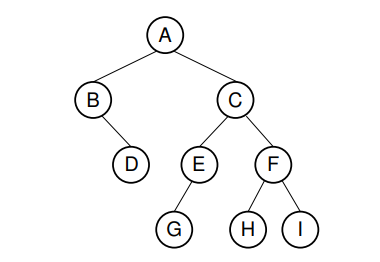
\includegraphics[scale = 0.8]{Capitoli/Alberi Binari/Esempi/Albero.png}
    
\end{center}
\textbf{in questa immagine abbiamo la rappresentazione di un albero binario}
\subsection{Profondità(Depth) e Altezza(Height)}
\begin{itemize}
    \item La \textbf{profondità} è la lunghezza del \textbf{path} da un nodo \textbf{M} a un nodo \textbf{N}. Tutti i nodi a \textbf{profondità d} risiedono al \textbf{livello d}
    \item \textbf{L'altezza è}: Partendo da un nodo \textbf{N} l'altezza è il numero di \textbf{archi} che devo attraversare per arrivare a una foglia(nodo più in profondità) quindi possiamo dire che l'altezza è \textbf{Depth}. il percorso valido verso le foglie è quello più lungo.
    \item la differenza tra \textbf{Depth} e \textbf{l'altezza} che sono inverse, scendendo \textbf{Depth} aumenta invece \textbf{l'altezza} diminuisce 
    \item il percorso valido verso le foglie è quello più lungo.
    \item Nel caso di un albero con un solo nodo allora si ha che la \textbf{Depth} e \textbf{l'altezza} sarà zero
    \item \textbf{P.S. :} La prof considera l'altezza come profondità + 1
\end{itemize}

\subsection{Nodi interni e foglie}
\begin{itemize}
    \item \textbf{Un nodo interno} è un nodo che ha almeno un figlio
    \item \textbf{Una foglia (leaf)} è un nodo senza figli
\end{itemize}
\subsection{Albero binario pieno}
\begin{itemize}
    \item Un albero è pieno quando per una certa altezza \textbf{h} ha il \textbf{numero massimo di nodi}, quindi ogni nodo interno ha sempre due figli.
\end{itemize}
\begin{center}
    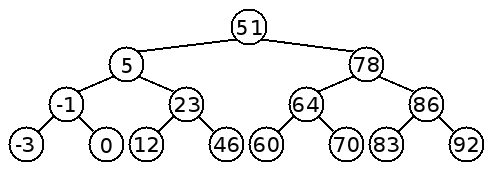
\includegraphics[scale = 0.6]{Capitoli/Alberi Binari/Esempi/AlberoPieno.png}
\end{center}
\newpage
\subsection{Albero binario completo}
\textbf{Un albero è detto completo se rispetta queste tre proprietà:}
\begin{enumerate}
    \item è un \textbf{albero binario}
    \item \textbf{le foglie} si trovano ad \textcolor{blue}{\textbf{altezza $h$ o $h-1$}}
    \item \textbf{al più un nodo} \textbf{\textcolor{blue}{interno}} può avere \textbf{meno di due figli}
\end{enumerate}
\begin{center}
    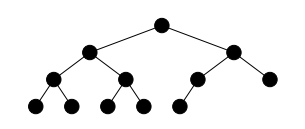
\includegraphics[scale = 0.8]{Capitoli/Alberi Binari/Esempi/alberocompleto.png}
\end{center}
\begin{tcolorbox}
    \textbf{\textcolor{blue}{NB:}} In questo corso per convenzione riempiamo un albero completo mettendo le foglie da \textbf{sinistra} verso \textbf{destra} in questo modo abbiamo la certezza che \textbf{tutti i livelli} siano pieni \textbf{eccetto} l'ultimo \textbf{livello} che può anche non essere pieno. L'albero di sopra rispetta questa proprietà.
\end{tcolorbox}

\subsection{Alberi binari Teoremi}
\textbf{un problema dei alberi binari} e che non c'è nessun vincolo di come io \textbf{posso posizionare} i miei dati, quindi può accadere che si crei una \textbf{catena}. In una struttura in cui i \textbf{dati sono solo} conservati nelle \textbf{foglie} questo potrebbe essere un grande problema poiché consuma molto spazio.
\begin{center}
    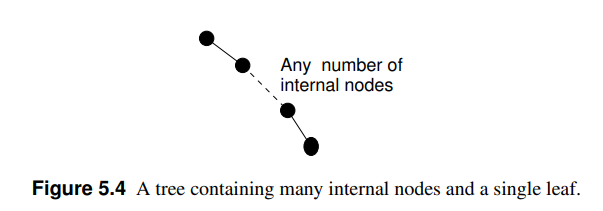
\includegraphics[scale = 0.6]{Capitoli/Alberi Binari/Esempi/catena.png}
\end{center}
\textbf{Per ovviare a questo problema ci sono molte altre famiglie di alberi binari come i alberi binari pieni un teorema molto importante ci dice:}
\subsubsection{Teorema: numero massimo di foglie in un albero pieno}
\textbf{\textcolor{blue}{Enunciato:}}\newline
\textit{Il numero di foglie in un albero pieno è uguale al numero di nodi interni più uno}\newline\newline
\newpage
\textbf{\textcolor{blue}{Dimostrazione:}}
\begin{itemize}
    \item Il teorema sarà dimostrato per induzione
    \item  \textbf{Caso base:} Per un albero altezza zero ($h = 0$) abbiamo che c'è solo una sola foglia, quindi i nodi interni sono: zero più uno è uguale a uno ($0+1 = 1$). Invece per altezza uno ($h = 1$) avrò un nodo interno , quindi uno più uno è uguale a 2 ($1+1 =2$), anche questa volta ci troviamo poiché essendo un albero pieno avremo due figli per l'unico nodo interno \textbf{(ovviamente un l'ipotesi è che stiamo lavorando su un albero binario pieno)}
    \item quindi osserviamo che sia per $h=0$ e $h = 1$ le nostra formula per calcolare le foglie è corretta cioè numero di nodi interni $n + 1$
    \item  \textbf{Ipotesi induttiva:} Ipotizziamo che ogni albero binario pieno $T$ abbia $n-1$ nodi interni e $n$ foglie.
    \item  \textbf{Passo induttivo:}
    Prendiamo un albero $T$ con $n$ nodi interni e prendiamo uno dei suoi nodi interni, lo chiamiamo $I$. Successivamente togliamo a questo nodo interno $I$ i due figli rendendolo cosi foglia. cosi facendo avremo un \textbf{sotto albero} $T'$ con $n-1$ nodi interni. Ora se prediamo $T'$ per la nostra ipotesi induttiva sappiamo che $T'$ ha $n$ foglie poiché ha $n-1$ nodi interni, se aggiungessimo a $T'$ le foglie che abbiamo tolto a $I$  cosa succederebbe? Avremo $T'$ con $n+2$ foglie, dobbiamo però toglierne una poiché la foglia a cui furono sottratti i figli ora è padre(non togliamo la foglia fisicamente ma solo dal conteggio), cosi avremo $n$ nodi interni e $n+1$ foglie. Abbiamo cosi dimostrato che anche aggiungendo due foglie(questo perché deve rimanere un albero binario pieno) avremo che il numero di foglie è il numero di nodi interni $+ 1$.
    
\end{itemize}
\subsubsection{Nodi pieni}
\begin{itemize}
    \item   \textbf{Un nodo è pieno} se ha due \textbf{figli} , se \textbf{non è pieno} è \textbf{foglia}(senza figli).
    \item  quindi ogni nodo o è \textbf{interno} o altrimenti è \textbf{foglia} non può avere un solo figlio.
\end{itemize}
\begin{center}
    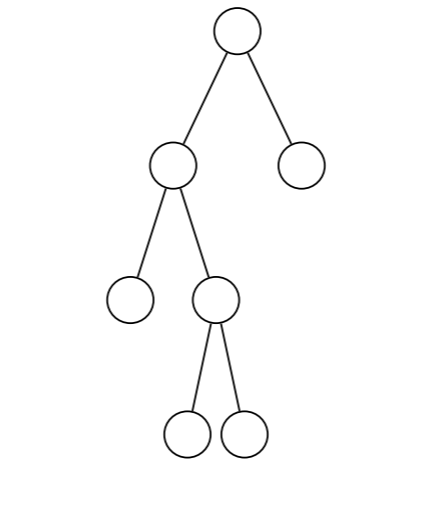
\includegraphics[scale = 0.3]{Capitoli/Alberi Binari/Esempi/NodiPieni.png}
\end{center}

\subsubsection{Definizione: alberi binari con figli non-vuoti e vuoti}
In questa immagine possiamo vedere che la figura (a) è un albero binario con la root con un foglio \textbf{sinistro} non vuoto, la figura (b)  è un albero binario con la root con un foglio \textbf{destro} non vuoto. Invece la (c)  è un albero binario con la root con il figlio \textbf{sinistro} vuoto, la (d)  è un albero binario con la root con il figlio \textbf{destro} vuoto
\begin{center}
    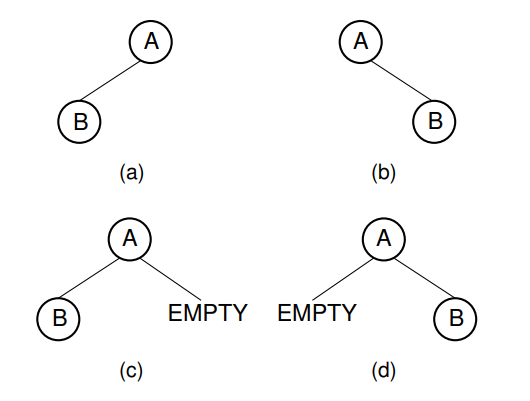
\includegraphics[scale = 0.5]{Capitoli/Alberi Binari/Esempi/Alberinonvuoti.png}
\end{center}
\subsubsection{Teorema: quanti sotto alberi vuoti ha un albero binario}
\textbf{\textcolor{blue}{Teorema}:} \textit{Il numero di  sotto alberi vuoti in un albero binario è il numero di nodi + 1}. \newline\newline
\textbf{\textcolor{blue}{Dimostrazione}:} Ogni albero binario $T$ ogni nodo ha due figli quindi per $n$ nodi un albero ha $2n$ figli dove $n$ è il numero di nodi. L'unico nodo senza parente è la root quindi possiamo dire che $n-1$ nodi hanno dei parenti.
sappiamo che $n-1$ nodi sono non vuoti. Togliendo al numero di figli totali il numero di nodi non vuoti ($n-1$) quindi otteniamo cosi $n+1$ che è il numero di sotto alberi vuoti poiché so che n-1 non sono vuoti

\newpage
\subsection{Modi di visitare L'albero}
\begin{itemize}
    \item \textbf{Traversal}: ogni processo per attraversare tutti i nodi in un certo ordine e che eseguono una specifica azione(es. stampare, sommare ecc.)
    \item Ogni \textbf{Traversal} che elenca ogni nodo \textbf{una sola} volta viene chiamata \textbf{Enumerazione(visita)}
    \item Gli \textbf{attraversamenti} possono seguire diversi ordini, tra cui:
    \begin{itemize}
        \item \textbf{\textcolor{blue}{Preorder}}: visito prima me stesso poi a sinistra e poi a destra.
        
        \item \textbf{\textcolor{blue}{Postorder}} : visito prima sinistra poi a destra e poi me stesso.
        
        \item \textbf{\textcolor{blue}{Inorder}}: visito prima sinistra poi me stesso e poi destra.
    \end{itemize}
    
    \begin{tcolorbox}[width=12cm, boxsep=10pt]
        \item \textbf{Esempio per contare nodi in un albero:}
        \lstinputlisting{Capitoli/Alberi Binari/Esempi/EsempioVisita.txt} 
    \end{tcolorbox}
\end{itemize} 
\subsection{Spazio richiesto per albero binario}
\begin{itemize}
    \subsubsection{Struttura}
    \item \textbf{Il nodo} deve contenere lo \textbf{spazio} per il dato e per i due \textbf{puntatori ai figli}
    \item \textbf{OverHead:} Il "overhead" per lo spazio di un albero si riferisce alla quantità di memoria aggiunta a quella utilizzata dai dati effettivi memorizzati nei nodi dell'albero.
    \item Quindi \textbf{l'overhead} è lo spazio richiesto per memorizzare tutto quello che non è il dato. quindi tutto quello che riguarda la struttura dati è \textbf{overhead}.
    
    \item  infatti \textbf{l'overhead} dipende da:
    \begin{itemize}
        \item in quale tipo di nodi memorizzo i dati (tutti, solo le foglie, . . . )
        \item se le foglie contengono comunque puntatori nulli
        \item se l’albero è a nodi pieni
    \end{itemize}
    \newpage
    \subsubsection{Spazio Richiesto}
    \item \textbf{Dato è piccolo}
    \begin{itemize}
        \item \textbf{\textcolor{blue}{Costo Totale:}} $n(2P + D)$ \newline\textbf{n} numero di nodi \textbf{P} sono i puntatori e \textbf{D} il dato
        \item \textbf{\textcolor{blue}{OverHead:}} $2nP$ senza il dato poiché è lo spazio richiesto in piu oltre al dato effettivo.
        \item \textbf{\textcolor{blue}{Percentuale di overhead:}} $2P/(2P + D)$ quindi se $P = D$ avrò il 2/3 di spazio che è \textbf{overhead}
    \end{itemize}
    \item \textbf{Se il dato è grande, nel nodo metto solo il puntatore}
    \item  Ho quindi tre puntatori, tutti di \textbf{overhead}:
    \begin{itemize}
        \item \textbf{\textcolor{blue}{Costo Totale:}} $n(3P + D)$ \newline\textbf{n} numero di nodi \textbf{P} sono i puntatori e \textbf{D} il dato
        \item \textbf{\textcolor{blue}{OverHead:}} $3nP$ senza il dato poiché è lo spazio richiesto in piu oltre al dato effettivo.
        \item \textbf{\textcolor{blue}{Percentuale di overhead:}} $3P/(3P + D)$ quindi se $P = D$ avrò il 3/4 di spazio che è \textbf{overhead}
    \end{itemize}

    \item \textbf{Se invece l'albero è pieno e non ho puntatori sulle foglie l'overhead è:}
    \begin{itemize}
        \item \textbf{\textcolor{blue}{Costo Totale:}} Avremo $2P + D$ per circa $n/2$ \textbf{nodi interni}.\newline Nelle foglie avremo $D$ per circa $n/2$ \textbf{foglie}. \newline\newline Quindi in totale avremo $\dfrac{n}{2}(2P+2D)$
        \item \textbf{\textcolor{blue}{OverHead:}} $\dfrac{n}{2}(2P)$
        \item \textbf{\textcolor{blue}{Percentuale di overhead:}} \newline\newline $\dfrac{\dfrac{n}{2}(2P)}{\dfrac{n}{2}(2P) + nD} = \dfrac{P}{P+D}$ 
        \item Se $D = P$ allora la percentuale di overhead è circa $1/2$
    \end{itemize}
\end{itemize}
\newpage
\textbf{\textcolor{blue}{Puntatori ai dati solo nelle foglie:}}
\begin{center}
    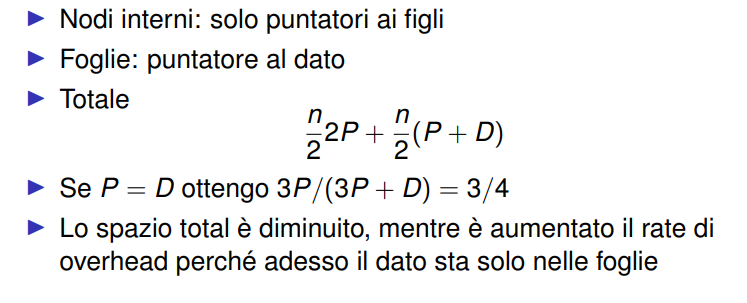
\includegraphics[scale = 0.7]{Capitoli/Alberi Binari/Esempi/DatoFigli.png}
\end{center}

\newpage
\subsection{Implementazione di un albero binario (Vettore)}
\begin{itemize}
    \item  Se conosciamo la struttura dell’albero, possiamo ridurre
    l’overhead legato ai puntatori.
    
    \item Se \textbf{l’albero binario è completo}, dato il numero di nodi \textbf{n} la
    sua struttura è unica.

    \item Questa \textbf{tecnica} funziona con i \textbf{alberi completi} poiché hanno un pattern ben preciso. Per funzionare questa tecnica ha bisogno che le foglie devono essere posizionate da \textbf{destra} verso \textbf{sinistra}.
    
    \item \textbf{Numero i nodi partendo dalla radice e scorrendo ciascun
    livello da sinistra verso destra in modo univoco}.
    
    \item \textbf{Questa numerazione mi dà la posizione all’interno
    dell’array:}

    \begin{itemize}
        \item \textcolor{blue}{\code{Parent(r)}} $= \left\lfloor \frac{r - 1}{2} \right\rfloor$ se $r \neq 0$
        \item \textcolor{blue}{\code{LeftChild(r)}} $= 2r + 1$ se $2r + 1 < n$
        \item \textcolor{blue}{\code{RightChild(r)}} $= 2r + 2$ se $2r + 2 < n$
        \item \textcolor{blue}{\code{LeftSibling(r)}}\textsuperscript{1} $= r - 1$ se $r$ è pari
        \item \textcolor{blue}{\code{RightSibling(r)}} $= r + 1$ se $r$ è dispari e $r + 1 < n$
    \end{itemize}
    \begin{center}
        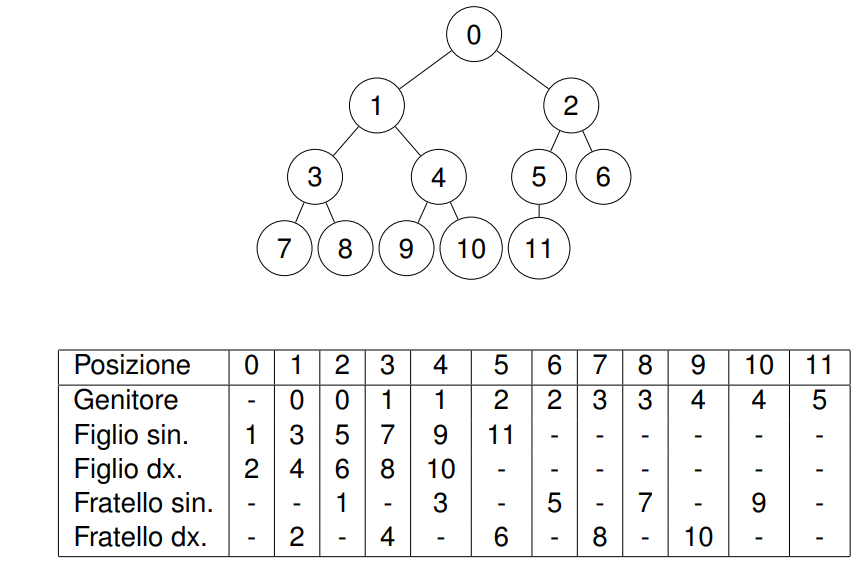
\includegraphics[scale = 0.6]{Capitoli/Alberi Binari/Esempi/AlberoFromArray.png}
    \end{center}
    \footnotetext[1]{Da il fratello Sinistro di $r$, se $r$ è il figlio destro LeftSibling(r) non restituisce nulla}
\end{itemize}

\section{Iteratori}
\begin{itemize}
    \item é un elemento che è in grado di indicare L'Elemento successivo in una struttura dati
    \item I Funzioni:
    \begin{itemize}
        \item  \textbf{\textcolor{blue}{\code{Lettura del dato nell’elemento;}}}
        \item  \textbf{\textcolor{blue}{\code{Controllo di terminazione;}}}
        \item  \textbf{\textcolor{blue}{\code{Successore (++);}}}
        \item  \textbf{\textcolor{blue}{\code{Ripristinare la radice}}} (ma solo nei \code{ResettableIterator}) o comunque il punto di inizio
    \end{itemize}
\end{itemize}

\subsection{Iteratori per i alberi}
Abbiamo diversi modi per visitare un albero:
\begin{itemize}
    \item \textbf{Visita in ampiezza}
    \item \textbf{Visita in profondità}
\end{itemize}
\subsubsection{Visita in ampiezza}
\begin{itemize}
    \item Abbiamo bisogno di una \textcolor{blue}{\code{coda}} di supporto per:
    \begin{itemize}
        \item \textbf{\textcolor{blue}{\code{Lettura del dato}}}: metodo della classe;
        \item \textbf{\textcolor{blue}{\code{Controllo di terminazione}}}: controlla se la coda è vuota;
        \item \textbf{\textcolor{blue}{\code{Sucessore}}}: Dequeue del nodo visitato e Enqueue dei due figli del nodo corrente.
    \end{itemize}
    \begin{center}
        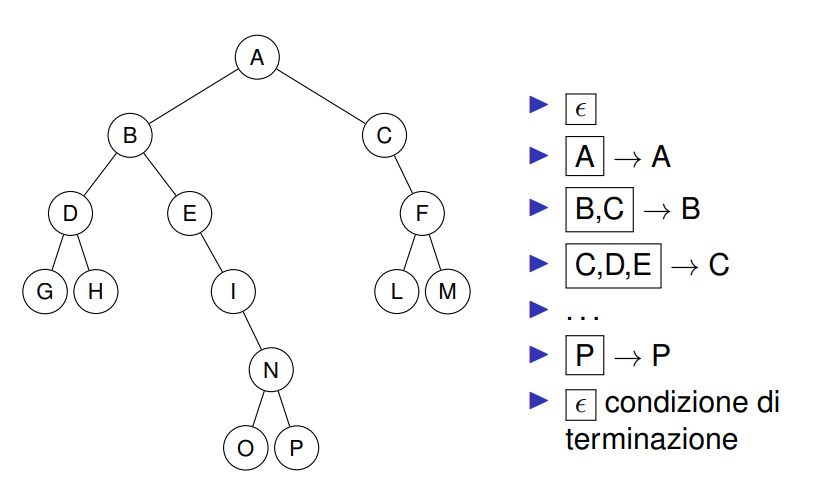
\includegraphics[scale = 0.5]{Capitoli/Iteratori/Esempi/Visita in ampiezza.png}
    \end{center}
\end{itemize}

\subsubsection{Visita in profondità}
Abbiamo tre modi per visitare in profondità:
\begin{itemize}
    \item \textbf{\textcolor{blue}{\code{Preorder}}}
    \item \textbf{\textcolor{blue}{\code{Inorder}}}
    \item \textbf{\textcolor{blue}{\code{Postorder}}}\newline\newline
\end{itemize}
Ci serve uno \textcolor{blue}{\code{Stack}} di supporto per la visita \textbf{\textcolor{blue}{\code{PreOrder}}}:
\begin{itemize}
    \item \textbf{\textcolor{blue}{\code{lettura del dato:}}} metodo della classe;
    \item \textbf{\textcolor{blue}{\code{controllo di terminazione:}}} \code{stack} vuoto;
    \item \textbf{\textcolor{blue}{\code{successore:}}} \code{Pop} del nodo visitato e \code{push} dei due figli del nodo corrente.
    \begin{center}
        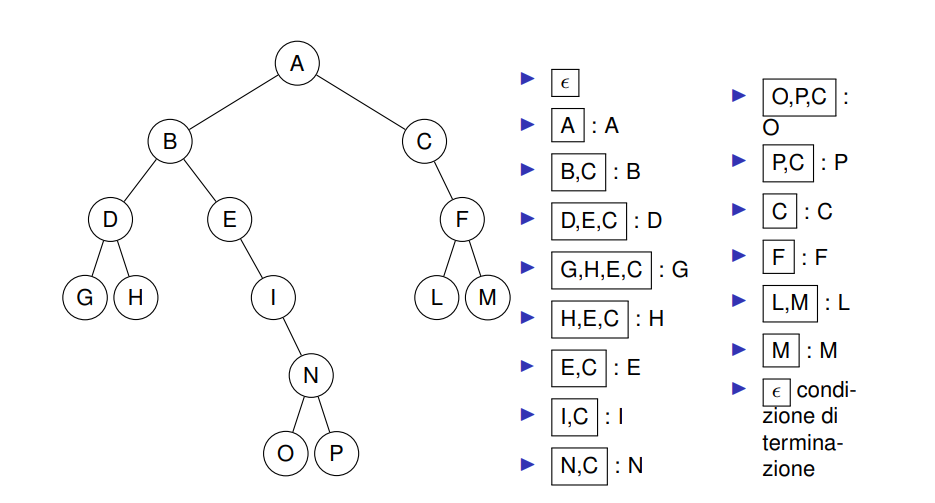
\includegraphics[scale = 0.6]{Capitoli/Iteratori/Esempi/visita PreOrder.png}
    \end{center}
    \begin{tcolorbox}[width=15cm, boxsep=10pt]
        \item \textbf{Codice Visita PreOrder:}
        \lstinputlisting{Capitoli/Iteratori/Esempi/CodicePreOrder.txt} 
    \end{tcolorbox}
\end{itemize}
\newpage
\textbf{Visita} \textbf{\textcolor{blue}{\code{InOrder}}}:
\begin{itemize}
    \item  In questo caso il \textbf{nodo corrente} viene scoperto, ma non
   \textbf{ ancora visitato}: prima bisogna visitare il \textbf{sottoalbero}
    \textbf{sinistro}.
    \item Solito \code{stack} di supporto.
    \item \code{searchLeftMostNode} Ci serve anche una funzione che
    continua a scendere a sinistra fino a quando possibile
    inserendo man mano i nodi che incontra nello stack: si
    ferma al primo nodo il cui figlio sinistro è vuoto.
    \item scopri Quando scopriamo un nodo, ne facciamo il \code{push}
    nello \code{stack} e poi scendiamo a sinistra con
    \code{searchLeftMostNode}
    \begin{itemize}
        \item \textbf{\textcolor{blue}{\code{lettura del dato:}}} metodo della classe;
        \item \textbf{\textcolor{blue}{\code{controllo di terminazione:}}} stack vuoto;
        \item \textbf{\textcolor{blue}{\code{successore:}}} Pop e restituisco il nodo; visita il suo nodo
        destro, se c’è.
    \end{itemize}
    \item Naturalmente parto dalla radice dell’albero.
    \begin{center}
        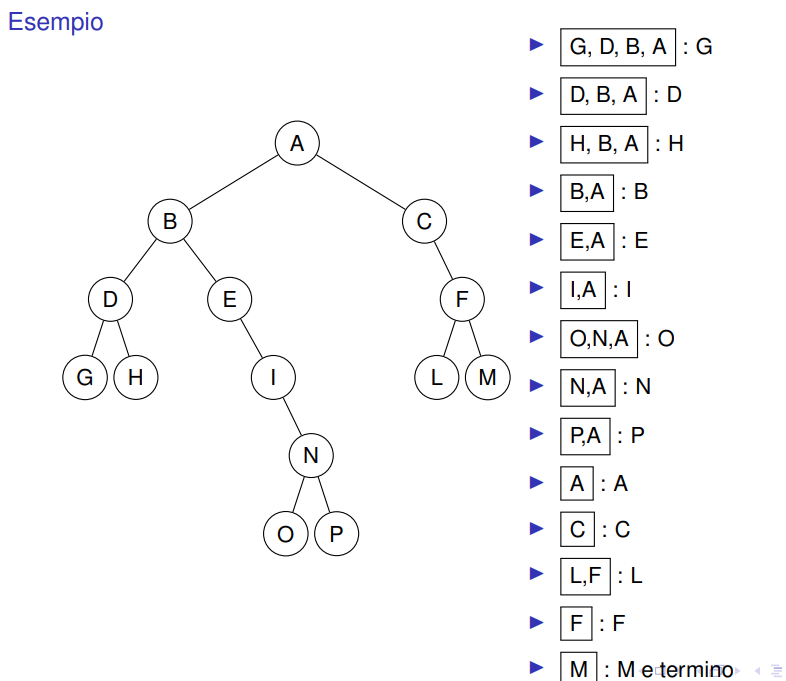
\includegraphics[scale = 0.6]{Capitoli/Iteratori/Esempi/Visita InOrder.png}
    \end{center}
\end{itemize}
\textbf{Visita} \textbf{\textcolor{blue}{\code{PostOrder}}}:
\begin{itemize}
    \item È un poi’ più complicato, perché la strategia cambia a
    seconda che stia risalendo l’albero da destra o da sinistra:
    per capirlo devo tenere l’ultimo nodo restituito, che
    chiameremo \code{current}.
    \item La visita di un nodo implica fare il \code{Pop} del nodo e poi
    scendere a sinistra con \code{searchLeftMostList}: quando
    trova un nodo col figlio sinistro vuoto, salta al destro e
    rincomincia a sinistra, fino a quando non trova una foglia.
    \begin{itemize}
    \item \textbf{\textcolor{blue}{\code{lettura del dato:}}} metodo della classe;
    \item \textbf{\textcolor{blue}{\code{controllo di terminazione:}}} \code{stack} vuoto;
    \item \textbf{\textcolor{blue}{\code{successore:}}} ripeti fino a quando non arrivi ad un \code{Pop} e
    restituisci:
        \begin{itemize}
            \item se \code{current == figlio sinistro} del \code{Top} dello \code{stack}, allora
            scopri il \textbf{figlio destro};
            \item se \code{current == figlio destro} del \code{Top} dello \code{stack}, \code{Pop} e
            \textbf{restituisci}
            \item altrimenti (foglia), \code{Pop} e \textbf{restituisci}
        \end{itemize}
    \end{itemize}
    \item Naturalmente parto dalla radice dell’albero.
    \begin{center}
        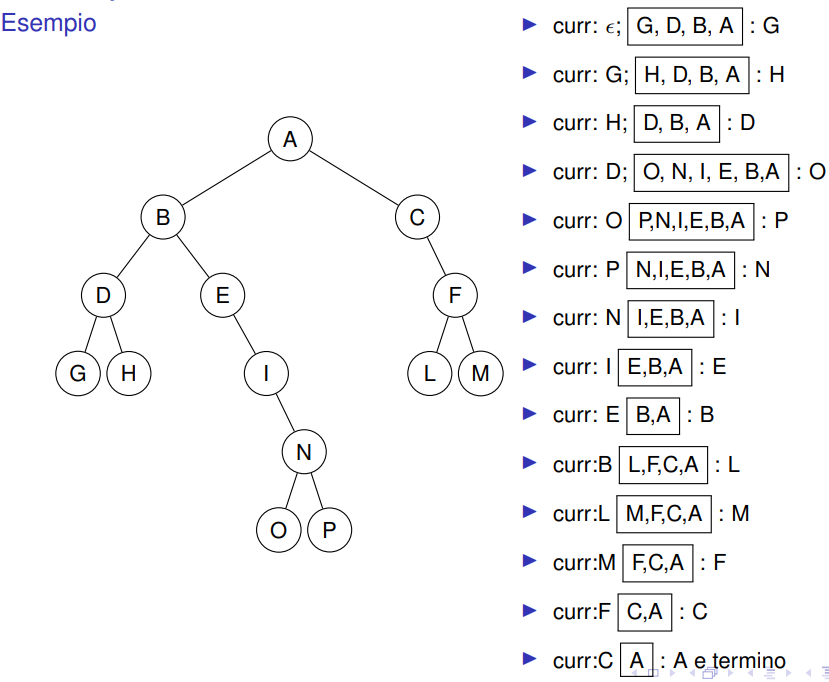
\includegraphics[scale = 0.5]{Capitoli/Iteratori/Esempi/Visita PostOrder.png}
    \end{center}
\end{itemize}
\newpage
\section{HashTable}
Le \textbf{hashtable} è un metodo per accedere alla array, il funzionamento è tramite delle chiavi(\textbf{keys}). Questo garantisce al momento della ricerca tempo constante poiché al record(l'informazione) è associata una chiave. Questa ricerca tramite la chiave per trovare il \textbf{record} viene chiamata anche \textbf{Hashing}.
I \textbf{record} vengono ordinati nel array in modo che \textbf{soddisfino il calcolo dei indirizzi}(cosi la ricerca nel array è più semplice). non sono ordinati per frequenza o valore.\newline\newline
\textbf{Terminologie:}
\begin{itemize}
    \item La funzione che mappa le chiavi e l'associa a una posizione nel array si chiami \textbf{\textcolor{blue}{\code{Hash function}}} denotato con \textbf{h}.
    \item  L'array che immagazzina i \textbf{recrod} viene chiamato \textbf{\textcolor{blue}{\code{Hash Table}}} e viene denotata con la parola \textbf{HT}
    \item Una posizione nella \textbf{hash tabele} viene chiamato \textbf{\textcolor{blue}{\code{slot}}}
    \item slot disponibili nella Hash Table viene denotato con \textbf{M}, i slot sono numerati da \textbf{0 a M-1}
    \item La \textbf{\textcolor{blue}{\code{Home}}} è l'indice restituito dalla \textbf{Hash function}.
\end{itemize}
l'obbiettivo per le \textbf{hash} è quello di organizzare le cose in modo che: Per ogni \textbf{K} chiave e una qualsiasi funzione \textbf{h} abbiamo che  $i =$ \textbf{h($K$)} dove $i$ è l'indice del array dove è immagazzinata l'informazione(\textbf{lo slot dove risiede il record}) della chiave \textbf{K}. la funzione \textbf{h} restituisce un valore tra $0 <= h(K) < M$. L'Obbiettivo è avere che \textbf{HT[i]} contiene il record della chiave \textbf{K}

\subsection{Debolezze generali}
\begin{itemize}
    \item Le \textbf{hashTable} non sono molto utili quando ci sono più \textbf{record} con la stessa chiave (quando permesso);
    \item \textbf{hashTable} non è molto efficiente a cercare in un determinato range
    \item non è efficiente a trovare il massimo o il minimo di un valore di una chiave oppure visitare i record in ordine di chiave
\end{itemize}

\subsection{Utilità}
\begin{itemize}
    \item Quando è utile ? quando vogliamo cercare ogni \textbf{record} con un certa chiave \textbf{K}. le hash vengono utilizzate per i database infatti vengono immagazzinate non solo sulla memoria centrale ma anche sulle memorie come hardisk o ssd.
\end{itemize}

\subsection{Osservazioni}
\begin{itemize}
    \item Nel caso ideale avremo un \textbf{hash table} con \textbf{M solt} e avremo delle chiavi \textbf{k} che vanno da \textbf{0 a M-1}. Cosi facendo avremo che con la chiave \textbf{k} nella \textbf{Hashtable} avrò \textbf{HT[k]} che contiene il \textbf{record} a cui è associato la chiave \textbf{k}. nel caso ideale usiamo tutti le chiavi. quindi a ogni chiave è associato un solo elemento.
    
    \item ovviamente questo se L'Intervallo delle possibili chiavi combacia con il numero di \textbf{slot}
    
    \item nel caso reale questo non avviene, se abbiamo che il range di chiavi è tra 0 e 65.535 dovremmo avere come minimo 65.535 slots però se abbiamo un aspettativa di utilizzare solo 1000 chiavi allora avremo altri 64.535 slots che non saranno mai utilizzatati.
    
\end{itemize}

\subsection{Risoluzione}
\begin{itemize}
    \item Quindi dobbiamo creare una funzione hash \textbf{h} che può mappare un grande intervallo di chiavi nel più piccolo numero di \textbf{slot} quindi in un \textbf{hash table} più piccola possibile.
    \item Questo perché di solito ci sono \textbf{sempre più possibili chiavi} che \textbf{slot}
\end{itemize}
\subsubsection{Problema(collisioni)}
\begin{itemize}
    \item Questa soluzione può portare a \textbf{collisioni} perché per due chiavi $K_1$ e $K_2$ po accadere che h($K_1$) $=$ $\beta$ $=$ h($K_2$)  dove $\beta$ è uno \textbf{slot} della \textbf{tabla hash}
    
    \item La ricerca di un record con valore chiave \textbf{K} in un database organizzato mediante\textbf{ hashing} segue una procedura in due passaggi: 
    \begin{itemize}
        \item 1. Calcolare la posizione della tabella \textbf{ h(K)}.
        \item 2. A partire dallo slot \textbf{h(K)}, individuare il \textbf{record} che contiene la \textbf{chiave} \textbf{K} utilizzando (se necessario) un criterio di \textbf{risoluzione delle collisioni}.
        
    \end{itemize}
  
\end{itemize}

\subsection{Funzione di Hash}
\begin{itemize}
    \item Lo scopo della \textbf{funzione Hash} è di utilizzare meno \textbf{slot} possibili per un certo \textbf{intervallo di chiavi}, ovviamente è impossibile evitare le \textbf{collisioni} in questo caso.
    \item in modo probabilistico meno \textbf{slot} abbiamo è più aumenterà la mobilita di \textbf{collisioni} poiché meno spazio disponibile. inoltre al aumentare delle chiavi aumenta di conseguenza la probabilità di \textbf{collisioni}.
    \item  quindi \textbf{diminuire} i slot e \textbf{aumentare} le chiavi aumenta le \textbf{collisioni}
    \item consideriamo, ad esempio, un'aula piena di studenti. Qual è la probabilità che una coppia di studenti condivida lo stesso compleanno (cioè lo stesso giorno dell'anno, non necessariamente lo stesso anno)? Se ci sono 23 studenti, allora le probabilità sono pari che due condivideranno lo stesso compleanno. Questo nonostante il fatto che ci siano 365 giorni in cui gli studenti possono avere compleanni (ignorando gli anni bisestili), nella maggior parte dei quali nessuno studente della classe compie gli anni. Con più studenti, aumenta la probabilità di un compleanno condiviso.
    
\end{itemize}

\textbf{Una funzione Hash si può considerare:}
\begin{itemize}
    \item \textbf{Indifferente:} va bene qualsiasi funzione che prende una
    chiave e restituisce uno slot.
    \item \textbf{Pessimo:} per qualsiasi chiave restituisce lo stesso slot: la
    tabella di hash non ci aiuta nella ricerca.
    \item \textbf{Ottimo:} ogni slot ha la stessa probabilità di venir colpito.
\end{itemize}

\subsection{Distribuzione delle chiavi}
\begin{itemize}  
    \item Per poter controllare la \textbf{distribuzione degli slot} (quante volte viene colpito uno slot o possibilità che un slot possa essere colpito), \textbf{dovremmo conoscere la distribuzione delle chiavi}(la possibilità che una chiave esca).
    \item Di solito conosciamo il range di valori che le chiavi
    possono assumere.
    \item A volte la distribuzione delle chiavi all’interno del range ci è
    favorevole:
    \begin{itemize}
        \item \textbf{Esempio} distribuzione uniforme delle chiavi(il che significa che ogni possibile chiave avrebbe la stessa probabilità di uscire): basta
        dividere il range in parti uguali.
        Questa frase si riferisce a un esempio di distribuzione uniforme delle chiavi all'interno di un certo intervallo di valori.

        Immagina di avere un intervallo di valori interi da \textbf{0 a 1000}
        e di voler distribuire le chiavi all'interno di questo intervallo in modo uniforme. \textbf{Dividere il range} in parti uguali significa che puoi suddividere l'intervallo totale in \textbf{segmenti} di uguale dimensione.
        
        Ad esempio, se vuoi distribuire le chiavi uniformemente su \textbf{10 segmenti o slot} \textbf{(o "parti uguali")}, puoi fare quanto segue:
        \begin{itemize}
            \item \textbf{Segmento 1:} da 0 a 100
            \item \textbf{Segmento 2:} da 101 a 200
            \item \textbf{Segmento 3:} da 201 a 300
            \item \textbf{Segmento 10:} 901 a 1000
        \end{itemize}
        Ogni segmento ha la stessa dimensione (in questo caso, 100) e contiene un decimo dell'intervallo totale di chiavi. Distribuire le chiavi in questo modo assicura che ogni segmento abbia la stessa probabilità di essere selezionato, garantendo così una distribuzione uniforme delle chiavi all'interno dell'intervallo.

    \end{itemize}
    
    \item Purtroppo la fortuna è rara, e in genere le chiavi risultano
    ammucchiate in alcune parti e rare altrove.
    \item In questi casi la scelta della funzione di hash è critica,
    \item ma dovrebbe partire dalla conoscenza della distribuzione
    delle chiavi.
\end{itemize}

\subsubsection{Perché distribuzioni non uniforme}
\textbf{avvolte le cattive distribuzioni non sono solo sfortuna:}
\begin{itemize}
    \item 1. Distribuzione di Zipf (Es: città grosse e piccole).
    \item 2. La raccolta dei dati introduce bias (Es: arrotondamenti dei
    numeri).
    \item 3. La prima lettera delle parole inglesi (e italiane e . . . ) non è
    uniforme.
\end{itemize}
\subsubsection{Esempi di funzioni di Hash}
\begin{tcolorbox}[width=15cm, boxsep=10pt]
    \textbf{16 slots:}
    \lstinputlisting{Capitoli/HashTable/Esempi/Es1HasFun.txt} 
    \begin{itemize}
        \item Lo slot dipende solo dai quattro bit meno significativi, che
        possono avere una cattiva distribuzione.
        \item Esempio di una scelta tipica: \%M: la scelta della
        dimensione della tabella di hash ha spesso un effetto
        importante sulle prestazioni.
    \end{itemize}
\end{tcolorbox}
\newpage
\textbf{Un altro esempio:}
\begin{itemize}
     \item Metodo mid-square:
    \item Fai il quadrato della chiave.
    \item Prendi gli $r$ bit centrali.
    \item Ottieni uno slot in $\left[0, 2^r - 1\right]$.
    \item Esempio:
    \begin{itemize}
        \item Chiavi: numeri decimali di 4 cifre.
        \item $M = 100$ (2 cifre decimali $\Rightarrow r = 2$)
        \item \textbf{Chiave}: 4567, al quadrato: 208\textbf{57}489
        \item Tutte le cifre contribuiscono a \textbf{57} quindi ci sarà più varianza e meno probabilità che esca lo stesso numero
    \end{itemize}
    \begin{center}
        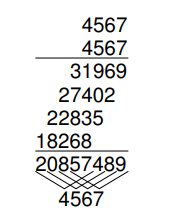
\includegraphics[scale = 0.8]{Capitoli/HashTable/Esempi/moltipilicazione.png}
    \end{center}

\newpage
    \subsection{Gestione delle collisioni}
    \item In pratica, le \textbf{collisioni} non possono venir escluse a priori,
    quindi vanno gestite.
    \item  Due classi principali, con:
    \begin{itemize}    
        \item \textbf{Hashing Aperto}(o con catene separate): le collisioni vengono immagazzinate fuori della tabella di   \textbf{hash}.
        \item  \textbf{Hashing Chiuso} : dentro la tabella di hash, in un altro slot
    \end{itemize}
    
\subsection{Open Hashing (indirizzamento chiuso)}
Nel \textbf{\textcolor{blue}{\code{Open Hashing}}} per ogni \textbf{slot} avremo un \textbf{record} , nel caso in cui ci fosse una \textbf{collisione} si creerebbe una lista \textbf{linkata}. in uno \textbf{slot} potremmo avere più \textbf{record} \textbf{linkati} fra di loro. \newline\newline
\textbf{Benefici:}
\begin{itemize}
    \item Questo metodo è molto semplice da gestire, di solito si può ordinare gli elementi della linked list tramite dei criteri, del tipo:
    \begin{itemize}
        \item Per numero di accessi
        \item Per ordine dei chiave
        \item a caso
    \end{itemize}
    \item  ovviamente dare un ordinamento può ritornare utile poiché il \textbf{tempo medio potrebbe beneficiarne}. se esempio accedo molto spesso alla chiave \textbf{"cane"} mediamente il mio $\theta$ medio sarà migliore.
\end{itemize}
    \begin{center}
        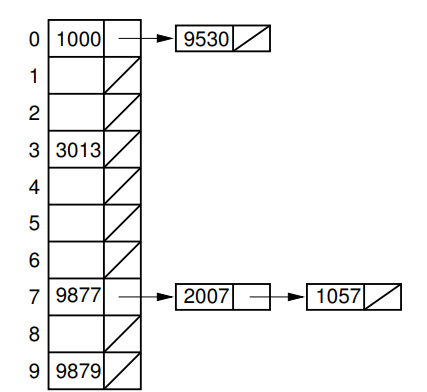
\includegraphics[scale = 0.6]{Capitoli/HashTable/Esempi/OpenHashing.png}
    \end{center}
\end{itemize}
\newpage
Se abbiamo \textbf{M} slot e \textbf{N} record da immagazzinare avremo che in ogni slot ci sarà $N \div M$. se invece stiamo nel caso in cui abbiamo \textbf{più slot} che \textbf{record} si spera che avremo \textbf{meno slot} possibili \textbf{con più di un record.} \newline
se ogni slot ha solo un record il tempo medio di accesso è $\theta(1)$.\newline\newline
\textbf{Svantaggi:}
\begin{itemize}
    \item La \textbf{linked list} o comunque delle strutture che hanno dei salti da un blocco al altro della memoria sono efficienti solo nella memoria primaria
    \item Nella \textbf{memoria secondaria} sarebbe poco efficiente poiché dobbiamo \textbf{accedere} più volte alla \textbf{memoria secondaria}(Sappiamo che la memoria secondaria è molto più lenta).
\end{itemize}
\subsection{Closed Hashing (indirizzamento aperto) Con Buckets}
\textbf{\textcolor{blue}{\code{{L'Hashing chiuso}}}} utilizza i \textbf{Buckets} quindi per\textbf{ M} slot e \textbf{B} buckets avrò che ogni \textbf{Bucket} avrà $M \div B$ slots. \newline
Ogni volta che la \textbf{Hash function} darà un indice questo sarà il numero del \textbf{bucket}. nel momento del inserimento del record dovrò partire dal inizio del \textbf{bucket} e scorrere finché non trovo uno slot libero. se il \textbf{bucket} è pieno il record sarà inserito in un \textbf{overflow bucket} che ha spazio "infinito"
\begin{center}
    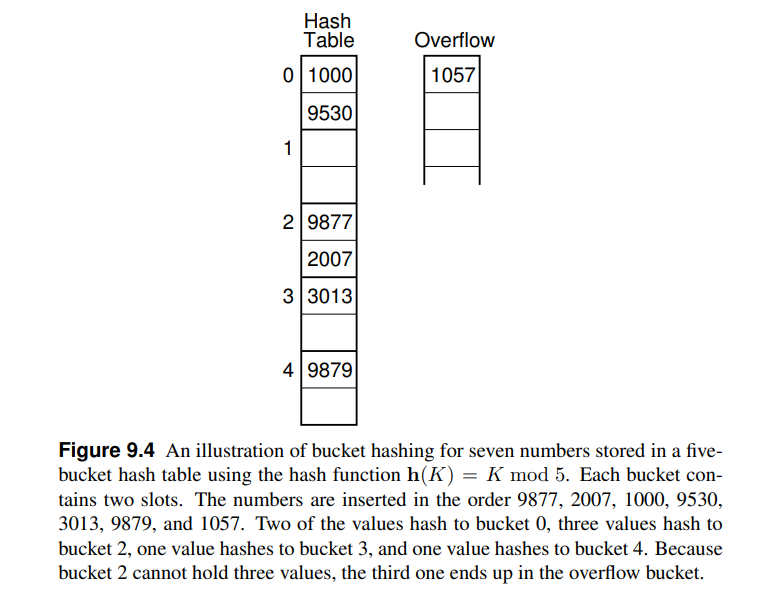
\includegraphics[scale = 0.6]{Capitoli/HashTable/Esempi/ClosingHash.png}
\end{center}
Una \textbf{buona} implementazione della \textbf{Hash function} e riempire sempre tutti i \textbf{bucket} e cercare di andare meno possibile nel \textbf{overflow bucket}

\subsubsection{Ricerca dei record}
Quando dobbiamo ricercare i record nel \textbf{HashTable} dobbiamo utilizzare la La \textbf{Hash Function} con la chiave \textbf{K} per determinare il \textbf{bucket}. Possiamo ricadere in vari casi:
\begin{itemize}
    \item Ricercare il \textbf{Bucket} dove risiede il \textbf{record} associato alla \textbf{chiave K}(la Chieve \textbf{K} ci serve a trovare il \textbf{bucket} tramite la \textbf{funzione di hash}, ma \textbf{K} ci servirà a trovare il corretto \textbf{record} nel \textbf{bucket}). Successivamente aver trovato il \textbf{bucket} si ricercherà il \textbf{record} con la chiave \textbf{K} nel \textbf{bucket}. Se \textbf{ricercando} troviamo una posizione vuota e non abbiamo ancora trovato il \textbf{record} allora quest'ultimo non è presente.
    
    \item Se ricercando  finisce il \textbf{bucket} dovremo andare in quello di \textbf{overflow}. per determinare se il \textbf{record} c'è oppure no dobbiamo navigare tutto il \textbf{bucket di overflow}
\end{itemize}

\subsubsection{Problemi e variante del bucket}
Il problema principale è che iniziando sempre a inserire dal primo elemento del \textbf{bucket} c'è più probabilità di \textbf{collisione} , di conseguenza più accessi da fare. Quindi accedo al primo slot se c'è \textbf{collisione} scendo al secondo slot , controllo il secondo slot se c'è \textbf{collisione} vado avanti ... e cosi via.\newline
\textbf{La variante}:
\begin{itemize}
    \item Quando inserisco un \textbf{record} accederò a uno \textbf{slot} \textbf{casuale} del \textbf{bucket} cosi diminuendo la probabilità di \textbf{collisione}
    \item Poi scorro finché non trovo una posizione libera, se arrivo alla fine del \textbf{bucket} risalgo al inizio e continuo , questa ricerca di inserimento finirà quando torno al punto di partenza.
    \item il \textbf{bucket} quindi è "circolare"
\end{itemize}
\begin{center}
    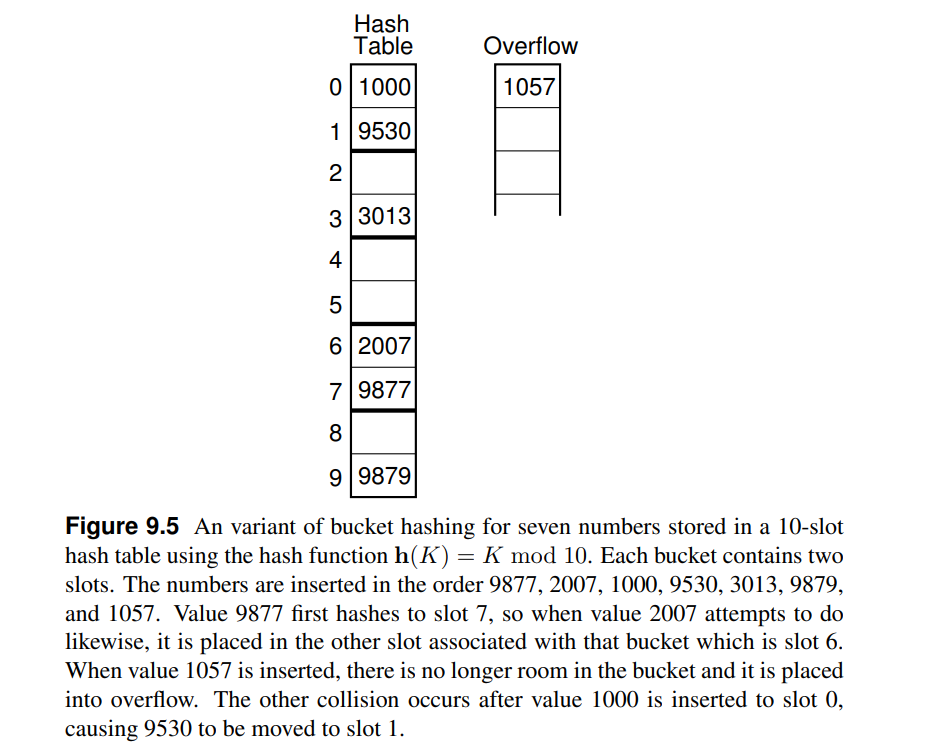
\includegraphics[scale = 0.6]{Capitoli/HashTable/Esempi/VarianteBuckets.png}
\end{center}
\newpage
\subsection{Closed Hashing (indirizzamento aperto) Con Linear Probing}
Questo metodo non ha i \textbf{bucket}. 
\subsubsection{Inserimento:}
Quando andiamo alla \textbf{Home} e accade una collisione durante l'inserimento si andrà a cercare nello slot successivo della \textbf{home}, se c'è uno \textbf{slot} libero si inserisce altrimenti si va avanti. Quindi \textbf{l'inserimento} cercherà dalla \textbf{home} in poi uno slot libero dove inserire l'elemento(La HashTable è circolare).\newline\newline
\textbf{Passaggi}:
\begin{itemize}
    \item Primo passo ottenere la \textbf{Home} con la funzione di \textbf{Hash}.
    \item Partendo dalla \textbf{home} trovare uno slot libero (\code{EMPTYKEY}) per ottenere \textbf{l'offeset} da aggiungere alla \textbf{home} si richiama la \textbf{probe function}( \textbf{P}$(K, i) = i$ dove $i$ è \textbf{L'offset})
    \item l'inserimento non parte propino se non ho almeno due slot liberi , questo perché lo slot libero ci servirà nella ricerca.
\end{itemize}
\begin{tcolorbox}[width=15cm, boxsep=10pt]
     \textbf{Inserimento}
    \lstinputlisting{Capitoli/HashTable/Esempi/InserimentoProping.txt} 
\end{tcolorbox}
La sequenza di slot dalla \textbf{Home} in poi viene chiamata  \textbf{\textcolor{blue}{\code{probe sequence}}} la funzione che restituisce \textbf{l'offset} da aggiungere alla \textbf{Home} è chiamata \textbf{\textcolor{blue}{\code{probe Function}}}
\newpage
\subsubsection{Ricerca}
Se si segue la \textbf{\textcolor{blue}{\code{probe sequence}}} la fase di ricerca è possibile. questo perché se nel inserimento non si  segue il \textbf{probe sequence} non abbiamo la sicurezza che se incontro uno spazio vuoto sono sicuro che la chiave \textbf{K} non c'è nella hash.\newline\newline
\textbf{Passaggi}:
\begin{itemize}
    \item Trovo la \textbf{Home} con la funzione di \textbf{Hash}
    \item Se la \textbf{home} non contiene \textbf{K} vado al successivo, quindi utilizzando la \textbf{probe Function} calcolo offset è vado avanti.
    \item mi fermerò quando lo trovo oppure quando trovo uno slot vuoto, questo indicherà che non c'è l'emento con chiave \textbf{K}
\end{itemize}
\begin{tcolorbox}[width=16cm, boxsep=10pt]
     \textbf{Ricerca}
    \lstinputlisting{Capitoli/HashTable/Esempi/RicercaProping.txt} 
\end{tcolorbox}
\newpage
\subsubsection{Primary Clustering}
Il \textbf{Proping primario} è il peggior metodo per risolvere le \textbf{collisioni}, perché soffre del \textbf{Primary Clustering}. Questo problema tende a far raggruppare due insieme di record. 
\begin{center}
    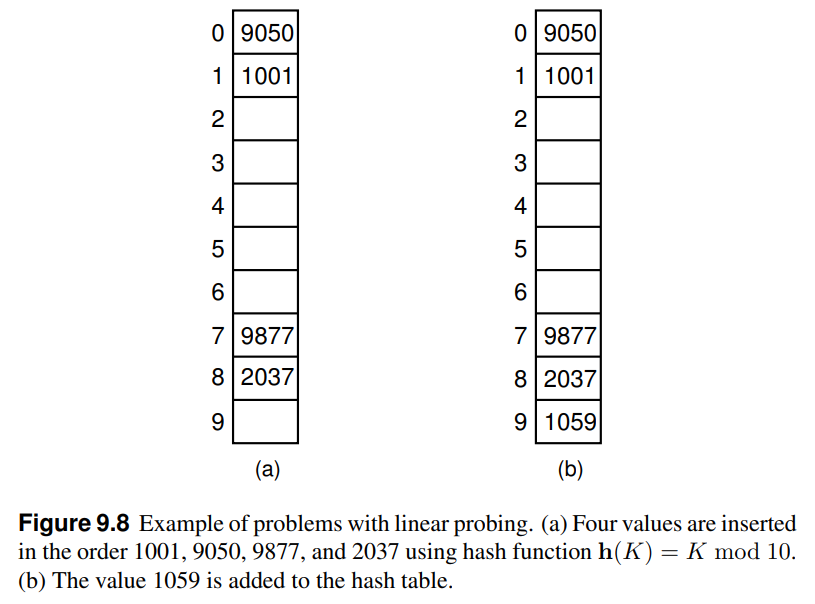
\includegraphics[scale = 0.36]{Capitoli/HashTable/Esempi/ClusteringPrimario.png}
\end{center}
Come notiamo nella figura sopra i due blocchi  si  tendono ad unirsi poiché le probabilità che il prossimo record sia inserito nella posizione \textbf{2} è del \textbf{0.6} quindi $6/10$ invece per tutti i \textbf{slot} da \textbf{3 a 6} è una possibilità su \textbf{10 quindi 0.1} \newline
questo perché se colpisco \textbf{7,8,9,0 o 1} andranno tutti a inserire nello \textbf{slot 2} poiché L'Inserimento andrà avanti finché non trova uno slot vuoto. 
\begin{enumerate}
    \item \textbf{Aumento del Tempo di Ricerca:}

    Quando si verifica clustering primario, le operazioni di ricerca richiedono più tempo perché più elementi devono essere esaminati. Se molte chiavi si trovano nello stesso cluster, bisogna scorrere una lunga sequenza di celle per trovare l'elemento desiderato.

    \item \textbf{Riduzione delle Prestazioni di Inserimento e Cancellazione:}

    Le operazioni di inserimento e cancellazione diventano meno efficienti perché richiedono il trattamento di collisioni. In presenza di un grande cluster, un nuovo elemento che collide con questo cluster deve essere inserito alla fine del cluster, aumentando così la lunghezza della sequenza.
    
    \item \textbf{Degradazione dell'Equilibrio della Tabella Hash:}

    L'accumulo di elementi in poche aree della tabella riduce l'efficacia della funzione di hash nel distribuire uniformemente le chiavi. Questo porta a un uso inefficiente dello spazio della tabella hash e può richiedere ridimensionamenti più frequenti.
    
    \item \textbf{Effetto Cascata:}

    Una volta che si forma un cluster, è probabile che questo cluster cresca più velocemente di altre aree della tabella, poiché le collisioni successive tenderanno ad aggregarsi ulteriormente al cluster esistente.
\end{enumerate}

\subsection{Miglioramento gestione collisioni (Hashing chiuso)}
Ci sono vari modi per risolvere il  \textbf{primary clustering}, il metodo più veloce è quello di aggiungere una costante moltiplicativa al \textbf{offset}.\newline
\begin{tcolorbox}
    \begin{itemize}
        \item Quindi la \textbf{\textcolor{blue}{\code{funzione di Proping}}} diventa nel seguente modo \textbf{P($K,i$)} $= ci$ dove \textbf{c} è la costante moltiplicativa.
        \item La \textbf{\textcolor{blue}{\code{probe sequence}}} sarà del tipo \textbf{(h($K$)$ + ic$) mod $M$}. il modulo di M per far in modo che il numero sia sempre al interno del numero di slot.
    \end{itemize}
\end{tcolorbox}
Un buona \textbf{\textcolor{blue}{\code{probe sequence}}} dovrebbe fare in modo che tutti i slot vengano visionati prima di ritornare alla \textbf{home}. Sfortunatamente in questo caso non è cosi.\newpage
\textbf{Esempio}
\begin{itemize}
    \item Se ho $c = 2$ , la home position  è pari e Il numero di slot M è pari allora avrò che capiterò sempre e solo sui slot pari, al contrario se la home position dispari andrò solo i quelli dispari.
    \item quindi non andrò mai a visionare tutti i slot ma solo una parte.
\end{itemize}
Essendo \textbf{M} variabile potrei avere dei problemi. Osserviamo che abbiamo \textbf{due blocchi}: il blocco dei  \textbf{numeri pari} e quello dei \textbf{numeri dispari}. Se uno dei due si riempisse troppo e l'altro rimarrebbe mezzo vuoto avremo che da una parte le\textbf{ prestazioni sono ottime} dal altro \textbf{pessime}. Questo non ci piace perché va a impattare in modo\textbf{ negativo} mediamente su tutta la struttura. Detto in poche parole il gioco non vale la candela!
\subsubsection{Risoluzione:}
Per risolvere questo problema basterà prendere una \textbf{c} che non abbia divisori in comune con la \textbf{M}(oppure prendere M primo) cosi facendo si prenderanno tutti i \textbf{solt}. Quindi se ho $M = 10$ , \textbf{c} dovrà essere \textbf{1,3,7} oppure \textbf{9}. Se invece $M = 11$ basterà un numero \textbf{tra 0 e 10}. Osserviamo che questo però non ci salverà dal \textbf{clustering primario} poiché con \textbf{c = 2} le chiavi $k_1$ e $k_2$ potrebbero avere una \textbf{\textcolor{blue}{\code{probe sequence}}} che converge nella stessa. Se \textbf{h($k_1$) = 3} la sequenza è \textbf{3,5,7,9} e cosi via. Se \textbf{h($k_2$) = 5} la sequenza è \textbf{5,7,9} e cosi via. come possiamo vedere dopo un certo punto è la stessa \textbf{\textcolor{blue}{\code{probe sequence}}}. in sintesi questo metodo non risolve il \textbf{clustering primario}

\subsubsection{Risoluzione Definitiva Clustering Primario}
Esistono due modi per risolvere \textbf{Clustering Primario} il primo  è avere un \textbf{offset} casuale , cosi facendo è statisticamente improbabile che due chiavi hanno la stessa \textbf{\textcolor{blue}{\code{probe sequence}}}. Questo è impossibile poiché  se avessimo un offset casuale non potremmo più ricercare un record poiché per una stessa chiave abbiamo un offset sempre diverso. Quindi posiamo usare dei numeri \textbf{pseudo-casuali}, questa tecnica viene chiamata \textbf{\textcolor{blue}{\code{pseudo-random probing}}}\newline\newline
\textbf{Funzionamento}:
\begin{itemize}
    \item Avremo quindi che \textbf{(h($K$) + $r_i$) mod $M$} sarà lo slot del inderimento/ricerca
    \item $r_i$ è il valore nella \textbf{i-esima} cella del vettore che conterrà valori casuali ma fissi, cioè dopo aver deciso i numeri casuali quest'ultimi non cambieranno. non sono valori casuali ma permutazioni dei valori da 1 a M-1.
    \item \textbf{\textcolor{blue}{\code{probe Function}}} è \textbf{p($K,i$) $=$ \code{Perm[$i-1$]}} dove \textbf{\code{Perm}} è un array di lunghezza \textbf{M-1} contando la \textbf{permutazione casuale} dei valori fa \textbf{ 1 a M-1}.
    \textbf{Quindi per chiavi diverse non avrò mai la stessa sequenza di probing.}
\end{itemize}
\begin{center}
    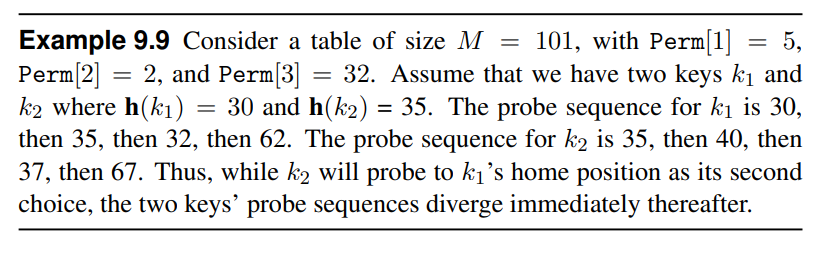
\includegraphics[scale = 0.6]{Capitoli/HashTable/Esempi/EsempioPseudo.png}
\end{center}
Il secondo metodo per risolvere il \textbf{clustering primario} è \textbf{\textcolor{blue}{quadratic probing}} dove la \textbf{funzione di proping} è \textbf{p($K,i$) $=$ $c_1 i^2 + c_2i + c_3$}. \newline
il caso più facile di è\textbf{ p($K,i$) = $i^2$} quindi \textbf{(h($K$) + $i^2$) mod $M$}
\begin{center}
    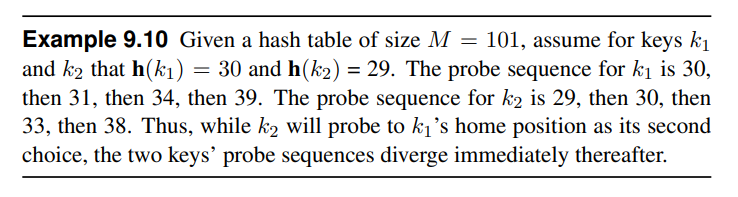
\includegraphics[scale = 0.6]{Capitoli/HashTable/Esempi/EsempioQuadratic.png}
\end{center}
il problema del \textbf{clustring quadratico} è che alcuni slot non verranno mai visionati, se per esempio avessimo una \textbf{hashtable} di \textbf{size 3} quindi abbiamo i slot \textbf{0,1 e 2} possiamo dire con certezza che \textbf{2} non sarà mai \textbf{visionato}. 
un modo semplice di risolvere è di avere \textbf{M} come numero primo cosi sicuramente meta tabella potrà essere riempita. oppure usare una \textbf{funzione di proping} del tipo \textbf{p($K,i$) $=$($i^2 + i$)/$2$} e M = $2^S$(M come potenza di 2) cosi facendo ogni \textbf{slot} sarà riempito.

\subsubsection{Clustering Secondario}
Il \textbf{\textcolor{blue}{\code{secondary clustering}}} si genera con le due nuove \textbf{funzione di proping}. Il \textbf{\textcolor{blue}{\code{secondary clustering}}} non genera dei cluster contigui ma delle \textbf{chiavi diverse} \textbf{K} possono avere la stessa \textbf{\textcolor{blue}{\code{probe sequence}}} e cosi facendo avendo dei cluster, però non contigui.
\begin{center}
    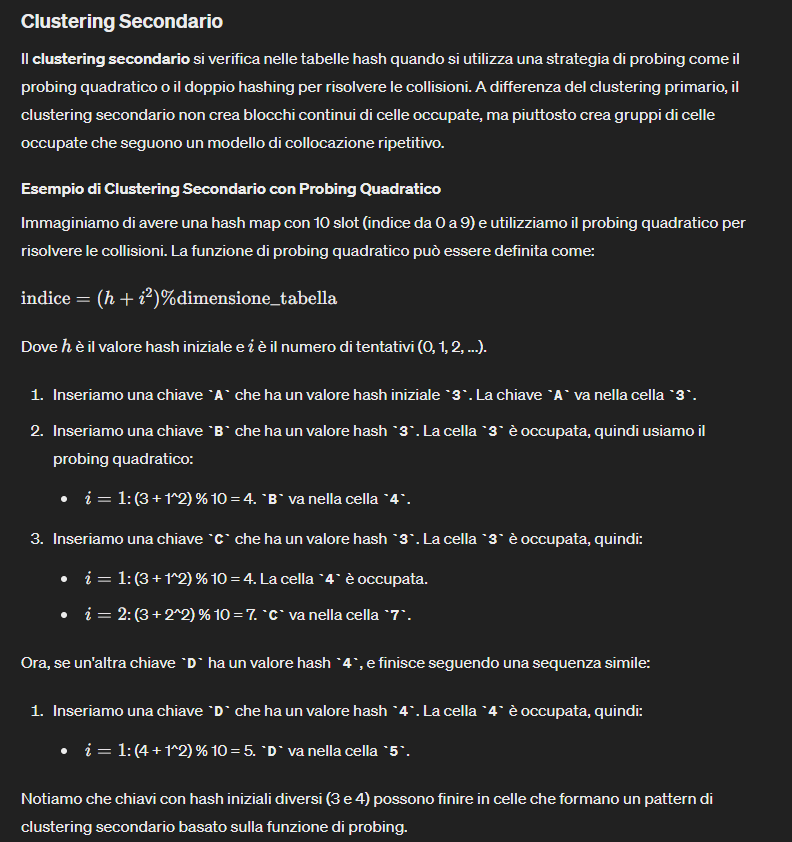
\includegraphics[scale = 0.8]{Capitoli/HashTable/Esempi/Esempio clustering.png}
\end{center}
\newpage
\subsection{Risoluzione Clustering Secondario}
Per risolvere il\textbf{ clustering secondario} si utilizza una \textbf{seconda funzione hashing} , il risultato di questa seconda funzione viene usata come \textbf{costante moltiplicativa}. quindi avremo \textbf{p($K,i$) $=$($i * h_2(K)$)}. questa $h_2$ restituisce un valore tra $1 <= h_2 <= M-1$
\begin{center}
    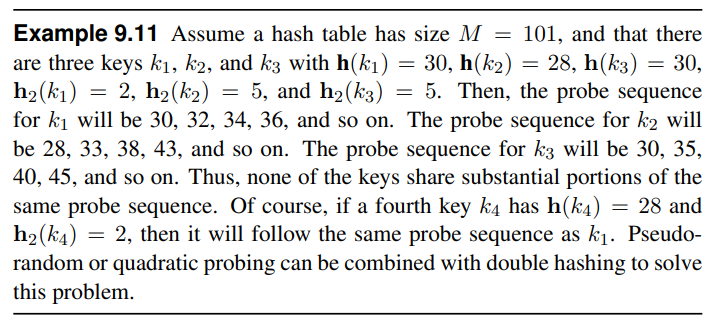
\includegraphics[scale = 0.6]{Capitoli/HashTable/Esempi/DoppioHashing.png}
\end{center}
questo ci garantisce di non avere \textbf{\textcolor{blue}{\code{probe sequence}}} uguali per chiavi diverse

\subsection{Risoluzione problema cancellazione}
La cancellazione deve affrontare due problemi:
\begin{itemize}
    \item \textbf{Cancellare un record} potrebbe creare dei problemi nella ricerca. Quando noi inseriamo un dato seguiamo una sequenza di \textbf{probing}, nel momento in cui \textbf{cancelliamo} un elemento potremmo rompere questa sequenza. Questo significa che nel inserimento siamo passati per un elemento che ora nella ricerca non c'è più(poiché cancellato) quindi troveremo uno \textbf{slot vuoto} prima del dovuto, cosi facendo non visiteremo tutta la sequenza di \textbf{probing}.
    \item  Il secondo problema che dobbiamo far in modo che lo slot che vogliamo cancellare sia riutilizzabile anche dopo la cancellazione 
\end{itemize}
\textbf{La risoluzione è molto semplice:} utilizzeremo delle \textbf{tombstone}(pietre tomabali). metteremo una \textbf{TombStone} quando cancelliamo, che sarà valutato come uno \textbf{slot pieno}nella ricerca, come \textbf{slot vuoto} nel inserimento. Quindi nel inserimento se \textbf{troviamo} una \textbf{tombstone} inseriamo, invece nella ricerca continuiamo.
\newpage

\subsection{Considerazioni}
Quindi quando si fa un \textbf{HashMap} si deve guardare:
\begin{itemize}
    \item Un ottima distribuzione dei slot quindi avere meno collisioni possibili
    \item una buona cosa di solito quando si vuole una ottima distribuzione è usare i \textbf{numeri primi}, poiché i \textbf{numeri primi} non hanno divisori in comune con nessuno. quindi i numeri che hanno gli stessi fattori produrranno valori \textbf{hash} con \textbf{pattern ripetitivi}. Usando un \textbf{numero primo}, si \textbf{riduce} questa ripetizione. questo perché si farà $h_1$(k) \% \textbf{M}
    \item  diciamo che per una distribuzione non uniforme delle chiavi dovrebbe ridurre il numero di collisioni
    \item ricordiamo che le chiavi nel caso reale non hanno una distribuzione uniforme.
\end{itemize}
\newpage
\section{Grafi}
Il grafo è un insieme di coppie di vertici dove:
\begin{itemize}
    \item $<V,E>$ Dove $E = \{A  \subseteq\ V | |A| = 2\}$  questo significa che \textbf{E} è un insieme formato da coppie di \textbf{vertici V}
    \item Possiamo indicare un grafo come \textbf{G} quindi possiamo scrivere $G = <V,E>$
    \item Quindi \textbf{E} è la \textbf{relazione binaria} su \textbf{V} ossia $E \subseteq V$x$V$ quindi \textbf{E} è L'insieme degli archi che sono presenti nel grafo \textbf{G}
    \item In un grafo \textbf{orientato} le coppie in \textbf{E} sono ordinate , quindi $(X,Y) \neq (Y,X)$ in un grafo \textbf{non orientato} questa differenza non c'è. 
    \item Diciamo che $0 \leq |E| \leq |V|^2 - |V|$, facciamo \textbf{meno |V|} poiché non considerammo i \textbf{self loop}
    \item Due vertici che hanno una \textbf{relazione} si chiamano \textbf{adiacenti}, quindi se abbiamo la coppia $(X,Y)$ allora \textbf{X e Y} sono adiacenti.
    \item Un \textbf{Grafo è etichettato} se ogni vertice ha una \textbf{"Etichetta"} che lo distingue dai altri.
    \item un \textbf{ciclo è semplice} se e solo se il primo è l'ultimo vertici sono uguali
    \item un grafo senza cicli viene chiamato aciclico 
    \item Il \textbf{grado massimo di un grafo} è il \textbf{numero massimo di archi uscenti da un nodo}
\end{itemize}
\subsection{Cammini}
\begin{itemize}
    \item Un percorso chiamato anche \textbf{Path} è una sequenza di vertici $v_0,v_1,...,v_n$ purché esistono dei archi tra questi vertici , quindi $(v_i,v_{i+1}) \in E$ dove $1 \leq i \leq n-1$
    \item Un \textbf{Path} è \textbf{Semplice} se tutti i vertici del percorso sono distinti
    \item La lunghezza del percorso è data dal numero di archi attraversati
    \item Un \textbf{Path} è \textbf{ciclico} se il \textbf{primo e l'ultimo vertice si ripetono}, un percorso per essere ciclico deve avere almeno una lunghezza $\geq 3$
\end{itemize}

\subsection{Sotto Grafi}
\begin{itemize}
    \item Presi Due grafi \textbf{G} e \textbf{G'} dove $G = <V,E>$ e $G'=<V',E'>$
    \item Diciamo che \textbf{G'} è un \textbf{sotto grafo} se $V' \subseteq V$ e $ E' \subseteq E$
    \item Dciamo che \textbf{G'} è un \textbf{sotto grafo indotto} se $V' \subseteq V$ e $ E' = E \cap V'$x$V'$
\end{itemize}

\subsection{Componenti concesse e fortemente connesse}
\begin{itemize}
    \item Un \textbf{grafo} o un \textbf{sotto grafo} \textbf{non orientato} si dice \textbf{connesso} se ogni vertice del grafo o sotto grafo può raggiungere tutti i altri 
    \item formalmente Se \textbf{G non orientato} si dice \textbf{connesso} se: \newline \[\forall v,w \in V | (V,W) \in Reach(G)\] \newline dove \textbf{Reach} è L'insieme di \textbf{coppie di vertici che sono raggiungibili } Quindi se abbiamo (V,W) significa che V raggiunge W e che W raggiunge V(dipende anche dal grafo)

    \item Un \textbf{grafo} o un \textbf{sotto grafo} \textbf{orientato} si dice \textbf{fortemente connesso} se ogni vertice del grafo o sotto grafo può raggiungere tutti i altri 
    \item formalmente Se \textbf{G orientato} si dice \textbf{fortemente connesso} se: \newline \[\forall v,w \in V | (V,W) \in Reach(G)\] \newline dove \textbf{Reach} è L'insieme di \textbf{coppie di vertici che sono raggiungibili } Quindi se abbiamo (V,W) significa che V raggiunge W e che W raggiunge V(dipende anche dal grafo)
    \item  Invece quando parliamo di \textbf{componenti} stiamo parlando di un \textbf{sottoinsieme massimale}, quindi \textbf{Componenti concesse e fortemente connesse} in più hanno solo che \textbf{sono massimali} 
\end{itemize}

\subsection{Metodi di Rappresentazione}
Abbiamo due metodi di rappresentazione di un grafo:
\begin{itemize}
    \item  \textbf{Tramite matrice di adiacenza}
    \item  \textbf{Tramite liste di adiacenza} 
\end{itemize}
\subsubsection{Matrice di Adiacenza}
\begin{itemize}
    \item Matrice \textbf{|V| × |V|} di bit: 1 se esiste l’arco, 0 altrimenti.
\item Per rappresentare matrici pesate, ogni elemento contiene
un numero.
\item In ogni caso, richiede spazio $\theta(|V|^2)$
\item Tempo richiesto per aggiungere o rimuovere un altro vertice è di $\theta(|V|^2)$ poiché devo \textbf{creare} una nuova matrice e poi copiare gli elementi della \textbf{vecchia alla nuova}
\item La ricerca di adiacenti di \textbf{un vertice} è \textbf{lineare su |V|} quindi $O(|V|)$, invece per una \textbf{visita completa} è $\theta(|V|^2)$
\item cancellazione di un arco è constante.
\end{itemize}
\subsubsection{Liste di Adiacenza}
\begin{itemize}
    \item Vettore di \textbf{|V|} liste linkate (o altri contenitori più adeguati): la
    lista nella posizione \textbf{i-esima} contiene i vertici adiacenti a $V_i$
    (e in questo modo rappresenta gli archi).
    \item il vettore piu li liste linkate richiedono uno spazio di $\theta(|V| + E)$, ovviamente perchè l'array di \textbf{|V|} più le  listelinkate che tutte insieme possono essere massimo \textbf{|E|}.
    \item Per aggiungere o rimuovere un vertice il costo sarà di $\theta(|V|)$ poiché si dovrà allocare un vettore e non una matrice
    \item Per una ricerca dei \textbf{ADJ} di un vertice è $\theta(|E|)$
    \item Per una ricerca di tutto il grafo allora $\theta(|V| + |E|)$ quindi  io navigo tutto l'array \textbf{|V|} , dopo aver visionato tutto il grafo avrò visitato \textbf{|E|} archi. Diciamo che la somma di tutte liste di adiacenza di ogni vertice è \textbf{|E|}
    \item La cancellazione di un arco non è più constante può essere nel caso peggiore $O(|E|)$ nel caso migliore $\Omega(1)$
    
\end{itemize}

\subsubsection{Quando usere Una matrice o una lista di adiacenza}
Un grafo si dice:
\begin{itemize}
    \item Il grafo è \textbf{Denso:} se il numero di archi si avvicina a $\theta(|V|^2)$
    \item Il grafo è \textbf{Sparso:} se il numero di archi è più o meno $\theta(|V|)$
\end{itemize}
Ci conviene usare una \textbf{matrice} se il grafo è \textbf{denso} poiché occuperemo meno spazio , questo perché la lista di adiacenza per colpa dei puntatori per una grande quantità di archi  avrà tanti puntatori e cosi pesando di più. \newline
Al contrario se un\textbf{ grafo è sparso} allora ci conviene usare le \textbf{lista di adiacenza}, poiché sprecheremo meno spazio.
\subsection{Metodi Accessori}
\begin{itemize}
    \item In genere gli algoritmi prevedono di visitare i nodi adiacenti
    al nodo dato.
    \item Daremo supporto a questa necessità con due funzioni:
    \begin{itemize}
        \item \textbf{\textcolor{blue}{first(v)}} restituisce il primo vertice adiacente al
        nodo \textbf{v}, quindi il primo della lista
        \item \textbf{\textcolor{blue}{next(v,n)}} restituisce il vertice adiacente a \textbf{v}
        immediatamente dopo n nella lista dei nodi
        adiacenti;\textbf{ n = |V|} a fine lista.
    \end{itemize}
\end{itemize}
\begin{tcolorbox}[width=14cm, boxsep=10pt]
    \lstinputlisting{Capitoli/Grafi/Esempi/scorimento_lista.txt}
\end{tcolorbox}
\newpage
\subsection{Visite}
\begin{itemize}
    \item Come per gli alberi, anche per i grafi esistono delle visite
    \textbf{(traversals)} standard.
    \item  Ogni vertice viene visitato una sola volta.
\end{itemize}

\subsubsection{Problemi}
\begin{itemize}
    \item \textbf{Due problemi principali:}
    \begin{enumerate}
        \item grafo \textbf{non connesso}: non è possibile raggiungere tutti i
        vertici da quello scelto per partire;
        \item presenza di \textbf{cicli}, che possono portare, se non controllati, a
        loop infiniti.
    \end{enumerate}

    \item  Entrambi i problemi possono venir \textbf{risolti} con dei \textbf{marcatori}
    sui vertici (un bit per vertice):
    \begin{enumerate}
        \item  \textbf{cicli}: evito di visitare vertici già visitati;
        \item  grafo \textbf{non connesso}: alla fine controllo per vedere se ci
        sono vertici ancora non visitati (se ci sono, riparto con la
        visita da uno di questi)
    \end{enumerate}

\end{itemize}

\subsection{Implementazione Visita}
Quindi per vistare tutti i vertici dobbiamo \textbf{scorrere tutto il vettore} è se il \textbf{vertice} \textbf{non è stato vistato} allora vistare tutti i suoi \textbf{ADJ}\newline
\begin{tcolorbox}[width=14cm, boxsep=10pt]
    \lstinputlisting{Capitoli/Grafi/Esempi/BaseVisita.txt}
    \begin{itemize}
        \item Dove \textbf{doTraverse()} può implementare una visita in \textbf{ampiezza o
        in profondità.}
    \end{itemize}
\end{tcolorbox}

\subsection{Visita in ampiezza(BFS)}
\begin{itemize}
    \item \textbf{Breath-first search (BFS).}
    \item Prima di procedere visiti tutti i vertici collegati al vertice
    corrente.
    \item Struttura di supporto: \textbf{coda}.
    \lstinputlisting{Capitoli/Grafi/Esempi/BFScodice.txt}
\end{itemize}
\begin{center}
    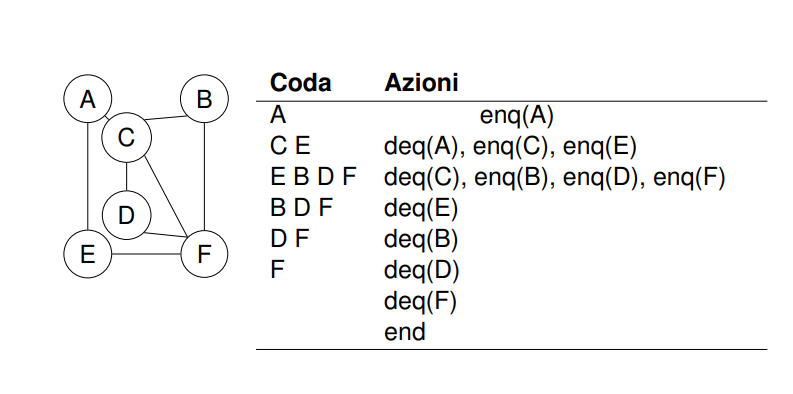
\includegraphics[scale = 0.6]{Capitoli/Grafi/Esempi/BFS.png}
\end{center}
\newpage
\subsection{Visita in profondità(DFS)}
Lo scopo della \textbf{DFS} è seguire il primo percorso del grafo finché non termina, nel momento in cui è terminato comincerà a risalire lo stack di esecuzione o di supporto finché non troverà una biforcazione. dopo aver trovato la biforcazione farà la stessa cosa che ha fatto al inizio , cioè percorrere tutto il percorso finché non termina. farà questo finché non visiterà tutto l'albero.
\begin{itemize}
    \item \textbf{Ricorsiva:} ogni volta che si visita un vertice \textbf{v} si visitano
    anche i suoi vicini non ancora visitati. però appena si trova un vicino non visitato entreremo in quel vicino e visteremo i suoi vicini, ripetiamo questo finché non troveremo nessun altro da esplorare
    \item \textbf{Iteratori}:
        \begin{itemize}
            \item si inseriscono in uno \textbf{stack} tutti gli archi che escono da \textbf{v};
            \item per \textbf{trovare il prossimo} vertice da visitare, si estrae e segue
            un arco dallo \textbf{stack}.
        \end{itemize}
        

    \item L’effetto è di seguire un ramo nel grafo fino alla sua
    conclusione prima di risalire le biforcazioni.
    \item Si costruisce così un \textbf{albero di ricerca in profondità.}
    \item \textbf{Vale sia per i grafi orientati che per quelli non orientati}
\end{itemize}
\newpage
\subsection{DFS Ricorsiva}
\lstinputlisting{Capitoli/Grafi/Esempi/DFSRicorsiva.txt}
\begin{center}
    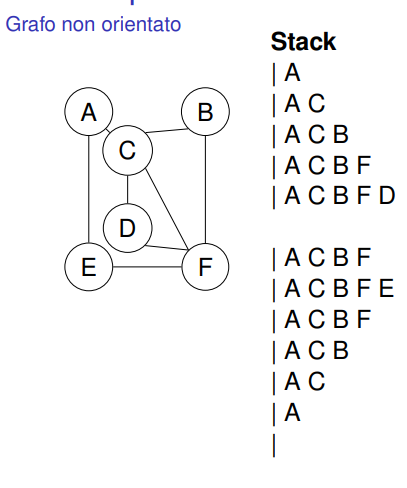
\includegraphics[scale = 0.6]{Capitoli/Grafi/Esempi/DFSNonOr.png}
\end{center}
\newpage
\subsection{DFS Iterativa}

\lstinputlisting{Capitoli/Grafi/Esempi/DFSIterativa.txt}
\begin{center}
    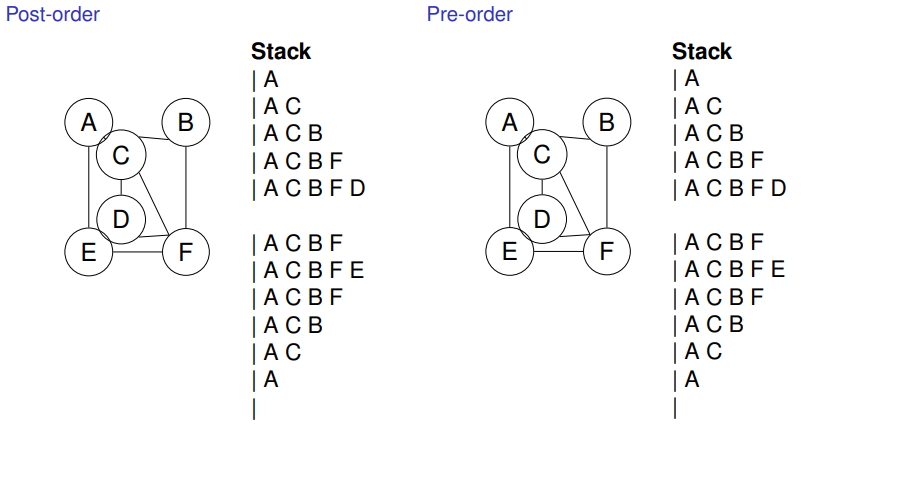
\includegraphics[scale = 0.6]{Capitoli/Grafi/Esempi/DFSIter.png}
\end{center}
Lo \textbf{stack non cambia} ma cambia solo l'ordine in cui viene effettuato il lavoro sul vertice

\newpage
\subsection{Foresta di visita}

\begin{center}
    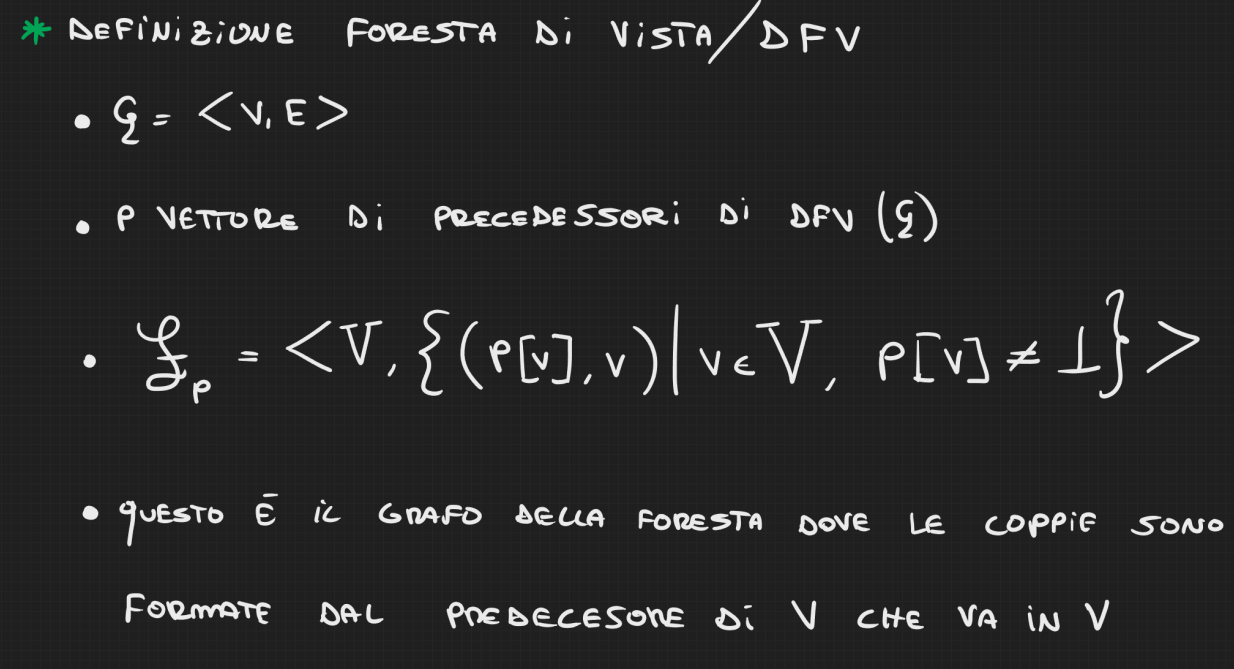
\includegraphics[scale = 0.5]{Capitoli/Grafi/Esempi/Foresta.png}
\end{center}
\subsubsection{Archi di Foresta}
\begin{center}
    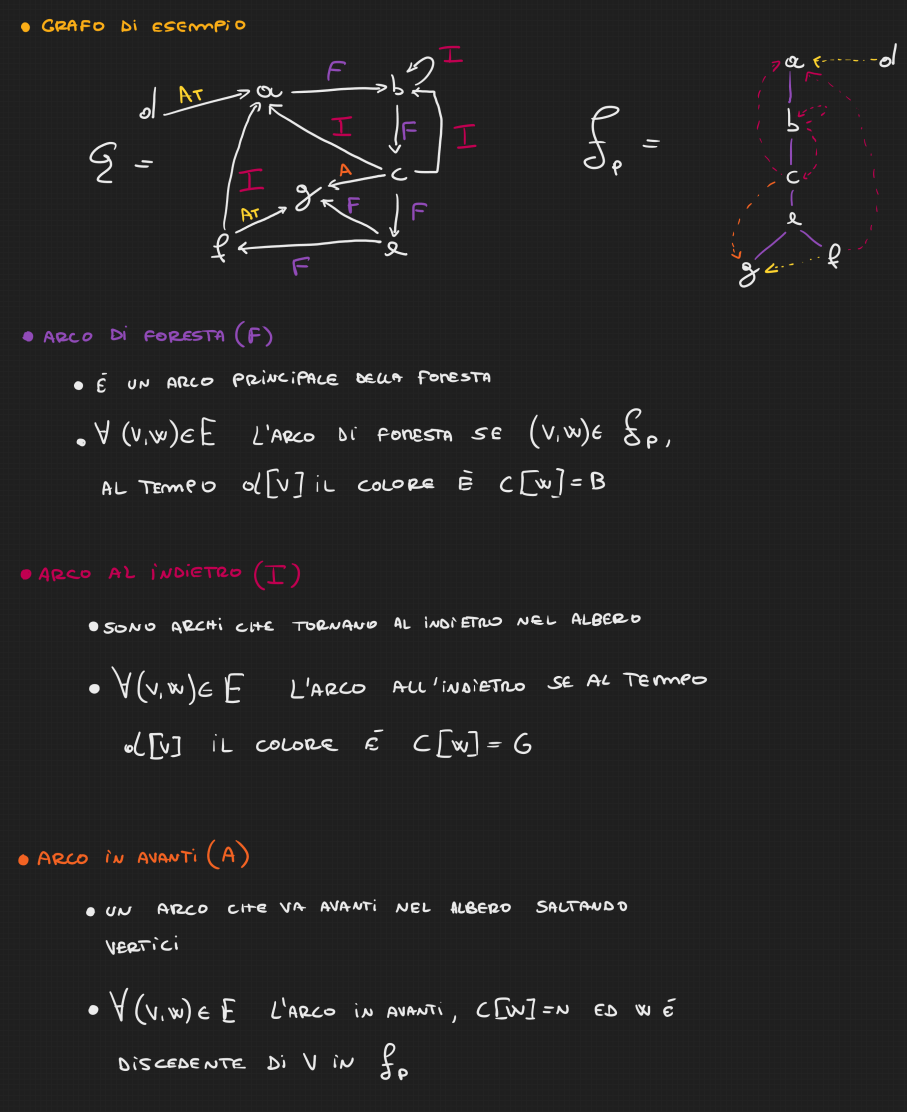
\includegraphics[scale = 0.6]{Capitoli/Grafi/Esempi/ArchiDiForesta.png}
\end{center}



\newpage
\section{Intercorso}
In questo paragrafo raggrupperò tutto quello che c'è da sapere sulle tre prove intercorso

\subsection{Using}
\textcolor{blue}{\code{\textbf{Using}}} è una \textbf{parola chiave} simile al \code{typedef} ma più versatile , si puo dire che è L'Evoluzione. \textcolor{blue}{\code{\textbf{Using}}} può essere usato per alias a:

\begin{enumerate}
    \item \textbf{Alias di tipo:} dare un nome a un tipo
    \begin{tcolorbox}[width=12cm, boxsep=10pt]
        \lstinputlisting{Capitoli/Intercorso/Esempi/Using/UsingTipe.txt}
    \end{tcolorbox}
    \item \textbf{Alias per le funzioni}: utilizzato per le funzioni anonime
    \begin{tcolorbox}[width=14cm, boxsep=10pt]
        \lstinputlisting{Capitoli/Intercorso/Esempi/Using/FunzioniAnonime.txt}
    \end{tcolorbox}
    \newpage
    \item \textbf{Alias di Namespace:} Dare nomi ai Namespace
    \begin{tcolorbox}[width=14cm, boxsep=10pt]
        \lstinputlisting{Capitoli/Intercorso/Esempi/Using/UsingNameSpace.txt}
    \end{tcolorbox}
    \item \textbf{Alias di tamplate:}
    \begin{tcolorbox}[width=14cm, boxsep=10pt]
        \lstinputlisting{Capitoli/Intercorso/Esempi/Using/UsingTamplate.txt}
    \end{tcolorbox}
\end{enumerate}

Quindi abbiamo 4 tipi di alias: \textbf{Tipo, funzioni, Namespace e tamplate}
\newpage
\subsection{lvalue e rvalue}
\subsubsection{lvalue}
Un \textcolor{blue}{\code{\textbf{lvalue}}} (left value) è un termine utilizzato in \code{C++} per descrivere un'espressione che rappresenta un \textbf{oggetto} che ha \textbf{un'identità} e un \textbf{indirizzo di memoria accessibile}. In altre parole, un \textbf{lvalue} è qualsiasi cosa che possa apparire alla sinistra di un'assegnazione (anche se non è l'unica caratteristica distintiva).\newline\newline
Caratteristiche di un \textbf{lvalue}:
\begin{itemize}
    \item \textbf{Ha un'identità}: Un lvalue rappresenta un oggetto che \textbf{risiede} in una \textbf{posizione} specifica nella \textbf{memoria.}
    \item \textbf{Può essere modificato}: Un lvalue \textbf{non const} può essere assegnato, quindi può essere modificato.
    \item \textbf{Può essere preso per riferimento}: Si può ottenere un \textbf{}riferimento a un lvalue.
\end{itemize}

 \begin{tcolorbox}[width=14cm, boxsep=10pt]
    \lstinputlisting{Capitoli/Intercorso/Esempi/lvalue e rvalue/lvalue.txt}
\end{tcolorbox}
\newpage
\subsubsection{rvalue}
In \code{C++}, un \textbf{rvalue} (right value) è un termine che descrive un'espressione che rappresenta un valore temporaneo, che non ha un'identità persistente o un indirizzo di memoria specifico. Gli \textbf{rvalue} sono tipicamente valori temporanei che non possono essere assegnati ad altre variabili (non possono essere lvalue).\newline\newline
Caratteristiche di un \textbf{rvalue}:
\begin{itemize}
\item \textbf{Temporaneità:} Gli \textbf{rvalue} sono valori che esistono solo per la \textbf{durata di un'espressione}.  \textbf{Non hanno un indirizzo di memoria stabile} a cui ci si può riferire dopo l'esecuzione dell'espressione.
\item \textbf{Non modificabili:} Gli rvalue non possono essere assegnati; puoi usarli per ottenere un valore, ma non puoi \textbf{modificarli direttamente}.
\item \textbf{Utilizzo in Espressioni:} Gli \textbf{rvalue} sono comunemente usati in espressioni matematiche, risultati di funzioni, e valori letterali.
\end{itemize}

 indichiamo un \textbf{rvalue} con \&\& (es. \code{f(Data \&\& s)} s è un rvalue)

 \begin{tcolorbox}[width=14cm, boxsep=10pt]
    \lstinputlisting{Capitoli/Intercorso/Esempi/lvalue e rvalue/rvalue.txt}
\end{tcolorbox}
\newpage
\subsection{std::move()}
\textcolor{blue}{\code{\textbf{std::move}}} è una funzione della libreria \textbf{standard di \code{C++}} che effettua il \textbf{cast} di un oggetto a un \textbf{rvalue reference}. Viene utilizzata principalmente per abilitare il trasferimento \textbf{(move)} di risorse da un \textbf{oggetto} a un \textbf{altro} senza \textbf{effettuare una copia}, ottimizzando così le prestazioni e l'efficienza della gestione delle risorse.\newline\newline
Cosa Fa \textcolor{blue}{\code{\textbf{std::move}}}?
\begin{itemize}
    \item \textbf{Cast a rvalue reference:} std::move effettua il \textbf{cast di un lvalue} (un oggetto con un nome e un indirizzo identificabile) a un\textbf{ rvalue reference}. Un \textbf{rvalue reference} è un tipo di riferimento che può essere legato a oggetti temporanei, permettendo l'implementazione delle semantiche di movimento.
    \item \textbf{Non Sposta Effettivamente:} std::move \textcolor{blue}{\code{\textbf{non sposta}}} effettivamente i dati o risorse; si limita a \textbf{indicare} che l'oggetto \textbf{può essere "spostato"}. L'effettivo spostamento delle risorse avviene nelle funzioni di movimento (\textbf{move constructor o move assignment operator}).\newline
\end{itemize}
 \begin{tcolorbox}[width=14cm, boxsep=10pt]
    \textcolor{blue}{\code{\textbf{NB:}}} Dopo un'operazione di \textbf{movimento}, l'oggetto sorgente è lasciato in uno \textbf{stato valido} ma \textbf{indeterminato}. Deve essere pronto per la distruzione, ma \textbf{non deve} essere usato ulteriormente senza essere \textbf{riassegnato} o \textbf{ricostruito}.\newline
    \textbf{No std::move su Oggetti Const} non ha senso.
\end{tcolorbox}
In sintesi, \textbf{std::move} è uno strumento potente per migliorare l'efficienza del codice \code{C++} consentendo il trasferimento delle risorse invece della loro copia.
\newpage
\lstinputlisting{Capitoli/Intercorso/Esempi/lvalue e rvalue/EsempioMove.txt}
\subsection{Lambada function}
Una \textbf{funzione lambda}, o \textbf{funzione anonima}, in \code{C++} è una funzione senza nome che può essere definita direttamente nel contesto in cui viene utilizzata. Le funzioni lambda sono state introdotte in C++11 e offrono una sintassi concisa per definire funzioni al volo, specialmente utili quando si lavora con funzioni di \textbf{ordine superiore}(es. fold, map ecc.).\newline\newline
La sintassi di base per una \textbf{lambda} in \code{C++} è la seguente:\newline\newline
\code{[ capture ] ( params ) -> return\_type \{ body \}}
\begin{itemize}
    \item \textbf{capture:} Specifica quali variabili del contesto circostante la lambda può catturare e utilizzare.
    \item \textbf{params:} Parametri della funzione lambda, simili a quelli di una funzione normale.
    \item \textbf{return\_type:} (Opzionale) Il tipo di ritorno della lambda. Se omesso, il compilatore deduce il tipo di ritorno.
    \item \textbf{body:} Il corpo della funzione lambda.
\end{itemize}
\lstinputlisting{Capitoli/Intercorso/Esempi/EsempiLambda.txt}
\newpage
\subsection{Problema del Diamante}
Il \textcolor{blue}{\code{\textbf{Problema del diamante}}} è un problema comune in linguaggi di programmazione orientati agli oggetti che supportano l'ereditarietà multipla, come \code{C++}. Si verifica quando una classe eredita da due classi base che a loro volta ereditano da una stessa classe base comune. Questa situazione può creare ambiguità su quale versione dei membri della classe base comune deve essere utilizzata, poiché esistono più \textbf{"percorsi"} per accedere a quei membri.\newline
Significa che quando in stanzio un oggetto e devo percorrere la strada verso il padre non saprò che strada percorrere.
\begin{tcolorbox}[width=14cm, boxsep=10pt]
    \textbf{Esempio:}
    \lstinputlisting{Capitoli/Intercorso/Esempi/Diamante/NonVirtual.txt}
    \begin{itemize}
        \item \textcolor{blue}{\code{\textbf{In questo esempio}}}, \code{DerivedFinal} eredita da \code{Derived1} e \code{Derived2}, entrambe ereditano da \code{Base}. Se proviamo a chiamare \code{obj.show()}, il compilatore non sa quale versione di \code{show} chiamare, quella ereditata da \code{Derived1} o quella ereditata da \code{Derived2}, perché ci sono due \textbf{percorsi} per arrivare alla funzione \code{show}.
    \end{itemize}
\end{tcolorbox}
\subsubsection{Risoluzione tramite virtual}
In \code{C++}, possiamo risolvere il \textcolor{blue}{\code{\textbf{Problema del diamante}}} usando \textbf{l'ereditarietà virtuale}. Con \textbf{l'ereditarietà virtuale}, diciamo al compilatore che ci sarà \textbf{una sola copia} della classe \code{base} condivisa tra tutte le classi derivate. \textbf{Questo elimina l'ambiguità}. elimina L'Ambiguità perché ci sarà solo una strada per la classe \code{base}.
\begin{tcolorbox}[width=14cm, boxsep=10pt]
    \textbf{Esempio:}
    \lstinputlisting{Capitoli/Intercorso/Esempi/Diamante/ConVirtual.txt}
    \begin{itemize}
        \item \textbf{Ereditarietà Virtuale:} Le classi \code{Derived1} e \code{Derived2} ereditano da \code{Base} usando \textcolor{blue}{\code{\textbf{virtual public Base}}}. Questo indica che \code{Base} deve essere condivisa tra tutte le \textbf{classi derivate} che utilizzano \textbf{l'ereditarietà virtuale}.
        \item \textbf{Ambiguità Risolta}: Ora, \code{DerivedFinal} ha una singola copia di \code{Base},\textbf{ eliminando l'ambiguità}. La chiamata a \code{obj.show()} funziona correttamente.
    \end{itemize}
\end{tcolorbox}\newpage
Quindi quando noi instanziamo una \textbf{classe} verrà instanziato anche la \textbf{classe} \textbf{padre}. Nel \textcolor{blue}{\code{\textbf{Problema del diamante}}} avevamo che una classe ereditava da due classi che avevano due istanze diverse della stessa classe padre(cioè \code{Base}). mettendo \textbf{virtual} usiamo la stessa istanza per entrambi.
\subsubsection{Quando usare l'Ereditarietà Virtual?}
L'ereditarietà virtuale è utile quando:
\begin{enumerate}
    \item \textbf{Si ha una gerarchia di classi con ereditarietà multipla}: Specialmente se si prevede che più percorsi di ereditarietà possano portare alla stessa classe base.
    \item  \textbf{Si desidera evitare copie multiple della stessa classe base}: Questo riduce il consumo di memoria e previene ambiguità.
\end{enumerate}
\newpage
\subsubsection{Funzionamento Tecnico}
Quando una classe \textbf{eredita un'altra classe in modo virtuale} oppure la classe che stiamo estendendo \textbf{contiene metodi virtuali} oppure la stessa classe contiene metodi virtuali allora abbiamo i seguenti tre componenti:
\begin{itemize}
    \item \textbf{vptr (puntatore alla tabella dei metodi virtuali)}: Ogni oggetto che contiene almeno un \textbf{metodo virtuale} (o \textbf{eredita} da una \textbf{classe con metodi virtuali}) ha un \textbf{vptr}. Questo \textbf{vptr} punta alla \textbf{vtable della classe stessa}.

    \item \textbf{vtable (tabella dei metodi virtuali)}: La \textbf{vtable} è una struttura dati globale per ogni classe che ha almeno un metodo virtuale. \textbf{Contiene i puntatori} ai metodi virtuali definiti per quella classe e per le sue classi base(da cui ha ereditato). Nel caso di un \textbf{OverRiding} il puntatore non punterà più a un metodo ereditato ma al metodo che lui stesso a fatto \textbf{L'override}. \textbf{vtable} non è una struttura dati globale nel senso che è condivisa tra tutte le istanze di quella classe. Ogni istanza della classe ha il proprio \textbf{vptr (puntatore alla vtable)}, che punta alla \textbf{vtable} specifica della classe stessa. vtable risolve le chimate a funzione quando c'è di mezzo metodi \textbf{virtual}.

    \item \textbf{Offset}: Gli \textbf{offset} per l'accesso alle classi base(quelle ereditate) \textbf{ereditate virtualmente} non sono direttamente memorizzati nella \textbf{vtable}. Questi \textbf{offset} sono \textbf{calcolati} dal \textbf{compilatore} e gestiti internamente per determinare l'indirizzo corretto dell'oggetto della classe base all'interno di un oggetto della classe derivata. Quindi nello \textbf{spazio} di \textbf{indirizzi logici} di un \textbf{istanza di una classe} risiede un \textbf{riferimento} per ogni \textbf{istanza di classe padre(classi da cui eredita)}, cosi facendo se più classi ereditano dalla stessa \textbf{non si crea ambiguità e ridondanza}, Quindi ci sarà un unica istanza per tutte L'istanze delle classi figlio. Per \textbf{raggiungere} questo riferimento \textbf{si usa l'offset}, quindi sommando \textbf{l'offset al indirizzo di base del oggetto ottengo il riferimento all'istanza della classe padre.}
\end{itemize}
\newpage
\subsubsection{Esempi:}
\lstinputlisting{Capitoli/Intercorso/Esempi/Diamante/CodiceEsempio.txt}
\newpage
\lstinputlisting{Capitoli/Intercorso/Esempi/Diamante/vtable1.txt}
Se togliessimo \textbf{foo} da D avremmo:
\lstinputlisting{Capitoli/Intercorso/Esempi/Diamante/vtable2.txt}
c'è \textbf{B} è non \textbf{C} poiché viene risolto prima \textbf{B} e poi \textbf{C} , questo perché \textbf{B} è stato scritto prima quindi in ordine di compilazione \textbf{B} viene risolto prima.
\newpage
\lstinputlisting{Capitoli/Intercorso/Esempi/Diamante/CodiceEsempio2.txt}
\lstinputlisting{Capitoli/Intercorso/Esempi/Diamante/vtableEs2.txt}
\end{document}
